% OARF — Online Anchor-Robust Forecasting under Economic Regime Shift
% Version submitted to Applied Stochastic Models in Business and Industry (transfer from JoF).
% Single-blind layout with author details and author-year references.
%
% Compile with: pdflatex manuscript && bibtex manuscript \
%   && pdflatex manuscript && pdflatex manuscript

\documentclass[12pt]{article}

% Compile with pdflatex. We deliberately keep the default OT1 text encoding so
% the body is set in the Computer Modern *Type-1* (vector) fonts that ship with
% a base TeX Live install. Loading [T1]{fontenc} without the lmodern or cm-super
% Type-1 EC fonts forces a bitmap Type-3 fallback for the running text, which
% renders as fuzzy/garbled glyphs in some PDF viewers; OT1 + cmap + glyphtounicode
% avoids that while still producing searchable, copy-pasteable ligatures.
\usepackage[utf8]{inputenc}
\usepackage{cmap}            % searchable/copyable ligatures
\input{glyphtounicode}
\pdfgentounicode=1
\usepackage[margin=1in]{geometry}
\usepackage{mathptmx}          % Times text and math (Type-1 fonts)
\usepackage{amsmath,amssymb,amsthm,bm}
\usepackage{graphicx}
\usepackage{booktabs}
\usepackage{array}
\usepackage{multirow}
\usepackage{caption}
\usepackage{subcaption}
\usepackage{xcolor}
\usepackage{enumitem}
\usepackage{algorithm}
\usepackage{algpseudocode}
\usepackage[section]{placeins}  % keep floats within their section
\usepackage[hidelinks]{hyperref}
\usepackage{xurl}               % allow long URLs to break across lines
\usepackage[round]{natbib}
\usepackage{authblk}

\graphicspath{{../figures/}}

\theoremstyle{plain}
\newtheorem{theorem}{Theorem}
\newtheorem{lemma}{Lemma}
\newtheorem{assumption}{Assumption}
\newtheorem{proposition}{Proposition}
\theoremstyle{remark}
\newtheorem{remark}{Remark}

\newcommand{\R}{\mathbb{R}}
\newcommand{\E}{\mathbb{E}}
\newcommand{\doop}{\mathrm{do}}
\newcommand{\OARF}{\textsc{OARF}}
\newcommand{\OARFCD}{\textsc{OARF-CD}}
\DeclareMathOperator*{\Var}{Var}
\DeclareMathOperator{\proj}{proj}

\title{\bfseries Online Anchor-Robust Forecasting under Economic Regime Shift}

\author[1]{Quang-Vinh Dang\thanks{Corresponding author. Email:
\href{mailto:vinh.dq4@buv.edu.vn}{vinh.dq4@buv.edu.vn}. ORCID:
\href{https://orcid.org/0000-0002-3877-8024}{0000-0002-3877-8024}.}}
\affil[1]{\small British University Vietnam, Hung Yen, Vietnam}

\date{\small Running title: Online anchor-robust forecasting}

\begin{document}
\maketitle

\begin{abstract}
\noindent
Forecasting models are fitted on past regimes, and they can fail when a driver such
as geopolitical risk or policy uncertainty moves to a level not seen before. Most
online methods respond after the shift, by detecting it and recalibrating. We study
whether a forecaster can be made robust in advance when the shift moves an observed
driver. OARF runs anchor regression online: it penalises the part of the forecast
error that is correlated with the driver, and with a zero penalty it is online
gradient descent. We prove a no-regret bound against a comparator evaluated under
the worst bounded shift of the driver. In simulations where the driver causes the
shift, OARF more than halves the worst-case error of online gradient descent, at
some cost in ordinary error, and stress tests show when the advantage disappears.
In weekly volatility forecasting for Brent crude and Henry Hub gas, every
combination method beats a persistence forecast, but OARF is no better than online
gradient descent or an equal-weight average. The method is therefore worth using
only when there is reason to believe that the chosen driver carries the shift, and
the paper describes checks that test this before deployment.

\vspace{0.6em}
\noindent\textbf{Keywords:} online learning; forecast combination; anchor
regression; structural change; volatility forecasting.
\end{abstract}

\section{Introduction}\label{sec:intro}

A forecasting model is estimated on data from the regimes it has seen. When a
geopolitical shock, a policy turn or an energy crisis moves the economy into a new
regime, relations that held in the estimation sample can break, and a model that was
well calibrated last month can be badly miscalibrated this month. The usual response
in online forecasting is to detect the break and adapt: monitor a loss or a coverage
statistic, raise an alarm when it drifts, then recalibrate or re-weight
\citep{gibbs2021aci,mfisher2025,watch2025}. This works, but the alarm can only fire
after the loss has risen, so the forecaster pays a re-adaptation cost at every break.

This paper asks a narrower question. Suppose the shift moves a variable that the
forecaster observes, such as an index of geopolitical risk, policy uncertainty or
market-wide volatility. Can the forecaster be built in advance so that its errors do
not depend on that variable, and what does this cost when no shift occurs? Anchor
regression \citep{rothenhausler2021anchor} answers this question for batch data. It
penalises the part of the residual that is correlated with a designated ``anchor''
variable, and under a linear structural model this is equivalent to minimising the
worst-case error over bounded shifts of the anchor. We make the estimator online and
test it on simulated and real forecasting problems.

\paragraph{An example.}
The following example shows what changes across regimes, what stays stable, and why
penalising the anchor helps. A target $y$, which could be next week's volatility, is
driven by a stable predictor $x_{\mathrm p}$: $y=x_{\mathrm p}+e_y$. A second predictor
$x_{\mathrm c}$ tracks the target but is also moved by an observed driver $a$:
$x_{\mathrm c}=y+a+e_c$. One can think of $x_{\mathrm c}$ as a news-based indicator
that rises with volatility but also with the volume of geopolitical headlines. In the
estimation sample $a$ has two regimes, with means $-1$ and $+1$. In the forecast period
its mean moves to $+3$, a level never seen in sample. The relation between $y$ and
$x_{\mathrm p}$ does not change; the relation between $y$ and $x_{\mathrm c}$ shifts by
the change in $a$. Table~\ref{tab:example} compares least squares with anchor
regression that uses $a$ as the anchor (the script is in the replication files). Least
squares puts some weight on $x_{\mathrm c}$, because in sample it carries information
about $y$, and it has the lower in-sample error. When $a$ moves to the new level that
weight becomes a liability, and the error of least squares roughly doubles. Anchor
regression sees that the residual of a predictor that leans on $x_{\mathrm c}$ moves
with $a$, removes that weight, and loses almost nothing in the new regime. It gives up
some in-sample accuracy ($0.240$ against $0.206$) in exchange.

\begin{table}[htbp]
\centering
\caption{The example of Section~\ref{sec:intro}. Weights and mean squared errors of
least squares and of batch anchor regression with penalty $\xi$, all fitted on the
two-regime estimation sample and evaluated on that sample and on a new regime in which
the mean of the driver $a$ moves from $\pm1$ to $3$ ($4{,}000$ draws in each sample).}
\label{tab:example}
\small
\begin{tabular}{lcccc}
\toprule
Method & weight on $x_{\mathrm p}$ & weight on $x_{\mathrm c}$ & MSE, estimation sample & MSE, new regime\\
\midrule
least squares             & $0.815$ & $0.176$ & $0.206$ & $0.452$\\
anchor regression, $\xi=10$  & $0.969$ & $0.021$ & $0.240$ & $0.242$\\
anchor regression, $\xi=100$ & $0.986$ & $0.003$ & $0.249$ & $0.247$\\
$x_{\mathrm p}$ alone     & $1$     & $0$     & $0.250$ & $0.248$\\
\bottomrule
\end{tabular}
\end{table}

The example also shows what the method needs. The anchor must be observed, and it
must be the variable through which the shift travels. If the analyst chose a variable
unrelated to the shift, the penalty would remove useful signal and buy no protection.
Sections~\ref{sec:synth} and~\ref{sec:real} measure how much of the benefit survives
when the anchor is noisy, misaligned or only weakly related to the shift.

\paragraph{What the paper does.}
Section~\ref{sec:method} turns the anchor-regression objective into a streaming
first-order update, \OARF{} (online anchor-robust forecasting), that uses
exponentially weighted moving averages of the relevant moments. With the penalty set
to zero it is online gradient descent, so one parameter controls how much in-sample
accuracy is traded for robustness. We define an interventional regret, in which the
comparator is evaluated under the worst bounded shift of the anchor, and prove that
the update is no-regret in this sense when the anchor is fixed. Section~\ref{sec:synth}
uses a simulated structural model in which the anchor causes the regime shifts, so
that robustness can be measured on shifts held out from training, and stress-tests the
method with noisy, misaligned and misspecified anchors. Section~\ref{sec:real} applies
it to weekly volatility forecasting for Brent crude and Henry Hub natural gas, with
macro-uncertainty indices as the anchor. Section~\ref{sec:learned} treats the case in
which the analyst does not know the anchor and describes a rule that estimates it from
the data, together with a check of when that estimate can be trusted.

The findings are mixed, and we report them as they are. In simulation, where the
anchor causes the shifts, \OARF{} more than halves the worst-case error of online
gradient descent, at a cost in ordinary error. The advantage disappears when the
anchor is observed with noise of about one standard deviation or is misaligned with the
true channel by more than about $50^\circ$, and it reverses when regimes shift
variances or the target equation itself. On the energy data, every combination method
beats a persistence forecast by a wide margin, but \OARF{} is not better than online
gradient descent or an equal-weight average, and the Model Confidence Set retains
almost all methods. The learned-anchor extension recovers the right subspace on most
simulated streams but fails badly on a minority, and its reliability check catches
most of those failures.

\section{Related work}\label{sec:related}

Our method draws on causal robustness, on online methods for distribution shift, and
on online convex optimisation.

\paragraph{Causal robustness and invariance.} The starting point is the observation
that a predictor which is \emph{invariant} across environments is also robust to
interventions that move between them. Invariant causal prediction
\citep{peters2016invariant} formalises this for the identification of causal
parents. Anchor regression \citep{rothenhausler2021anchor} turns it into an
estimator. By penalising the projection of the residual onto an anchor variable, it
interpolates between ordinary least squares and an instrumental-variables solution,
and the penalised problem is provably equivalent to minimising worst-case risk over
a bounded set of interventions on that anchor. DRIG \citep{shen2023drig} extends
the principle to distributional robustness through invariant gradients. All of
these are batch procedures that take the environment or anchor variable as given,
which is the obstacle for a streaming deployment. \OARF{} keeps the
worst-case-intervention interpretation of anchor regression and makes the estimator
online. We also study a heuristic add-on that estimates the anchor channel from
data. Because that estimate can be unreliable, we pair it with an online diagnostic
that flags streams on which the learned channel should not be used; on those streams
the forecaster reverts to plain online gradient descent. Our theorem covers only the
fixed, analyst-supplied channel. For a deployment that cannot supply one, the
diagnostic is a partial safeguard.

\paragraph{Reactive online adaptation.} A second, very active line of work treats
distribution shift as something to detect and then accommodate. Adaptive conformal
inference \citep{gibbs2021aci} adjusts a miscoverage level online to maintain
coverage under drift. Methods from 2025 tighten the detect-then-adapt loop
considerably. M-FISHER \citep{mfisher2025} maintains an exponential test martingale
over non-conformity scores and, when the martingale crosses a Ville threshold,
takes a Fisher-preconditioned natural-gradient correction. WATCH/WCTM
\citep{watch2025} monitors a weighted conformal test martingale that tolerates
benign covariate shift while still flagging harmful concept shift, and adapts the
prediction interval accordingly. These are the incumbents against which a proactive
method should be judged. \OARF{} tests whether, when an informative anchor is
available, the need for reactive triggering can be partly reduced by removing the
channel's influence before it raises the loss.

\paragraph{Distributionally robust forecasting.} The closest competitors are
recent methods that, like \OARF{}, optimise an explicitly worst-case objective.
\citet{wang2026online} propose online randomised distributionally robust forecast
combination for dependent data. They draw combination weights from a distribution
over the simplex and update it by stochastic mirror descent on a Wasserstein
ambiguity objective. \citet{liu2026fcdro} develop adaptive robust combination with
variance- and Expected-Shortfall-scaled exponential weights for yield-curve
forecasting, and \citet{chen2026wdro} analyse Wasserstein distributionally robust
online learning as a primal--dual game with regret guarantees. A parallel strand
makes conformal decisions cost-sensitive \citep{costaci2026}. Several of these
2025--2026 works are recent preprints, so we treat them as contemporary literature
and competitive baselines, not as settled, peer-reviewed results. They differ from
\OARF{} in geometry. They hedge over an \emph{isotropic} ambiguity ball centred at
the empirical distribution, which spreads robustness equally in all directions,
including directions along which the data never shift. \OARF{} hedges over the
anchor-shaped ellipsoid $\E[aa^\top]$, so its robustness budget is spent only
along the anchor directions in which shifts occur. Our experiments are designed to
isolate this difference. They show that the anchor-shaped geometry improves
interventional robustness when the anchor is informative, and that the gain shrinks
or reverses when it is not.

\paragraph{Adjacent online and subspace methods.} Nearby work also informs our
design. Online invariant and domain-adaptation methods seek predictors that hold
across changing environments in a streaming setting. \OARF{} can be seen as an
online, single-anchor instance of this idea, specialised to mean-shift
interventions, with a closed-form robustness term in place of an explicit
environment partition. Nonstationary-subspace and change-adaptive analysis
(subspace tracking, stationary-subspace analysis, and the path-length-adaptive
online learning of \citealp{zhang2018adaptive}) is what our discovery layer does:
it is an unsupervised nonstationary-subspace estimator, and for that reason we do
not call its output causal. What separates \OARF{} from these methods is that it
feeds the discovered nonstationary subspace back into an anchor-regression
objective whose target is interventional, not purely predictive.

\paragraph{Online convex optimisation.} The regret analysis rests on dynamic-regret
results for online gradient descent \citep{zinkevich2003ogd,hazan2016oco}, the
path-length-adaptive refinement of \citet{zhang2018adaptive}, and AdaGrad-style
preconditioning \citep{duchi2011adagrad}. The economic measurements draw on the
daily Geopolitical Risk index \citep{caldara2022gpr}, the Economic Policy
Uncertainty index \citep{baker2016epu}, realised-volatility modelling in the
heterogeneous-autoregressive tradition \citep{corsi2009har}, and the
volatility-timing logic of \citet{fleming2001voltiming}.

\section{The OARF method and its guarantee}\label{sec:method}

\paragraph{Setup and protocol.}
We work in discrete time $t=1,\dots,T$. At each step the forecaster observes
predictors $x_t\in\R^d$ and a vector of candidate regime drivers $z_t\in\R^p$, and
must predict a scalar target $y_t$. In a pure forecasting problem the predictors are
explanatory variables; in a combination problem they are the forecasts of several
base models. A linear predictor with feature map
$\phi(x)=[1;x]\in\R^{d+1}$ and weights $w$ emits $\hat y_t=w^\top\phi(x_t)$, incurs
the squared loss $\ell_t(w)=(y_t-\hat y_t)^2$, and writes its residual
$r_t=y_t-\hat y_t$. The \emph{anchor} is a (possibly learned) linear read-out of the
context, $a_t=B^\top z_t\in\R^q$, with channel matrix $B\in\R^{p\times q}$. The learning protocol is sequential. At step $t$ we first predict from $x_t$, then reveal $y_t$ and update, and each learner standardises its inputs with past-only statistics. When we later evaluate a frozen learner on held-out interventions, we replay the same frozen standardiser.

\paragraph{Objective.}
Following anchor regression \citep{rothenhausler2021anchor}, \OARF{} trades
predictive fit against invariance of the residual to the anchor by minimising
\begin{equation}\label{eq:bar}
b_{\mathrm{AR}}(w;\xi) = \underbrace{\E\!\big[(y-w^\top\phi(x))^2\big]}_{\text{predictive loss}}
 + \xi\,\underbrace{\E[a r]^\top\big(\E[aa^\top]\big)^{-1}\E[a r]}_{P(w)=\|\proj_a r\|^2},
 \qquad \xi\ge 0 .
\end{equation}
The penalty $P(w)$ is the squared length of the projection of the residual onto the
anchor. Driving it down forces $\E[a r]\to 0$, so the predictor stops using any
component of the signal that co-moves with the regime drivers. At $\xi=0$ the
objective is ordinary least squares, and as $\xi$ grows the solution moves toward the
invariant predictor. The objective also has a robustness interpretation.

\begin{proposition}[Interventional-robustness equivalence,
\citealp{rothenhausler2021anchor}, Thm.~1]\label{prop:equiv}
Assume a linear structural causal model in which (a) the anchor $A$ is a
\emph{source} (exogenous) node; (b) the remaining variables, including the target,
follow linear structural assignments $V=\mathbf{B}V+\varepsilon+\mathbf{M}A$ with
$A\perp\varepsilon$ and $I-\mathbf{B}$ invertible; (c) the considered interventions
are mean-shift interventions $\doop(a:=\nu)$ that replace $A$ by a constant; and (d)
the loss is squared error. Then for every $\xi\ge 0$ there is a radius
$\rho(\xi)$, given in closed form by the cited theorem and strictly increasing in
$\xi$ (with $\rho(0)=0$, the OLS support, and $\rho(\xi)\!\to\!\infty$ as
$\xi\!\to\!\infty$, the instrumental-variables limit), such that
\begin{equation}\label{eq:equiv}
\min_w b_{\mathrm{AR}}(w;\xi) \;=\; \min_w\ \sup_{\nu:\,\|\nu\|\le\rho(\xi)}\
 \E_{\,\doop(a:=\nu)}\!\big[(y-w^\top\phi(x))^2\big].
\end{equation}
\end{proposition}
\noindent The equivalence does not hold for arbitrary nonstationarity. It requires the
exogenous-anchor SCM (a)--(c) above, and the worst case is taken over mean-shift
interventions only. Under these conditions the set hedged over is an ellipsoid shaped
by the anchor covariance $\E[aa^\top]$, whereas the distributionally robust methods of
Section~\ref{sec:related} hedge over an isotropic ball; our evaluation tests whether
this difference in geometry matters. Our theory inherits the same assumptions
(Assumption~\ref{ass:scm}). Where they fail, the stress tests of
Section~\ref{sec:synth} measure the degradation.

\paragraph{Streaming update.}
The gradient of \eqref{eq:bar} in the coefficient block separates into a prediction
term and a robustness term,
\begin{equation}\label{eq:grad}
\nabla_w b_{\mathrm{AR}} = -2\,\E[\phi r]
 \;-\;2\xi\,\E[\phi a^\top]\big(\E[aa^\top]\big)^{-1}\E[a r],
\end{equation}
and to move from batch to streaming we replace each population moment by an exponential
moving average (decay $\beta$) of its sample analogue, computed on centred variables.
Subtracting the running means removes the across-regime mean component of the anchor.
Under the SCM of Proposition~\ref{prop:equiv}, where a regime is a mean shift on $A$,
this is the component that varies between regimes, and what remains is the
within-regime second-moment structure used by the penalty in \eqref{eq:bar}.
Centring does not remove the intervention itself, whose effect persists in $X$ and
$Y$. It only keeps the slowly varying regime mean out of the covariance estimate. The
channel-discovery rule of Section~\ref{sec:learned} uses the across-regime mean
variation that centring discards. Writing $\tilde\cdot$ for the EMA-centred quantities, and
collecting the non-intercept coefficients as $w_{-0}$, we maintain running estimates
$m^{Xr}_t$, $m^{XA}_t$, $M^{AA}_t$, $m^{Ar}_t$ of
$\E[\tilde\phi\,\tilde r]$, $\E[\tilde\phi\,\tilde a^\top]$,
$\E[\tilde a\tilde a^\top]$, $\E[\tilde a\tilde r]$ (here $\tilde\phi$ stacks the
intercept and centred $\tilde x$, and the intercept row of $m^{XA}_t$ is held at
zero so the penalty never acts on the intercept), and update
\begin{equation}\label{eq:update}
\boxed{\;w_{t+1}=w_t-\eta\,g_t,\qquad
 g_t=\underbrace{-\,r_t\,\phi(x_t)}_{\text{prediction}}
 \underbrace{-\,2\xi\,[\,0;\,m^{XA}_t(M^{AA}_t+\epsilon I)^{-1}m^{Ar}_t\,]}_{\text{anchor robustness}}
 +\,\lambda_2[0;w_{t,-0}].\;}
\end{equation}
Of the two factors of $-2$ in \eqref{eq:grad}, the prediction one is absorbed into
the step size $\eta$ and the robustness one is kept explicit, so that $\xi$ reads
directly as a relative weight. Signs follow gradient descent: the ridge term
$+\lambda_2[0;w_{-0}]$ enters $g_t$ with a positive sign, and the update
$w\!\leftarrow\!w-\eta g_t$ therefore shrinks the non-intercept weights. The ridge
$\epsilon$ stabilises the anchor Gram matrix $M^{AA}_t$ when it is ill-conditioned (we
use $\epsilon=10^{-3}$). Each step costs $O(d+pq+q^3)$, dominated by the $q\times q$
solve, which is negligible for the small $q$ we consider. In practice we take the step
with AdaGrad per-coordinate scaling \citep{duchi2011adagrad}. The gradient $g_t$ is
exactly \eqref{eq:update} and only its step length is preconditioned, so the
online-convex-optimisation regret machinery is unchanged, while a single global rate
adapts to features on very different scales. With $\xi=0$, $g_t$ reduces to the plain
squared-loss gradient and the update is online gradient descent; this holds
regardless of AdaGrad and standardisation, which act identically on all methods. The
decay $\beta$ controls how quickly the moment estimates forget.

\begin{algorithm}[t]
\caption{\OARF{}, one streaming pass. The block for learning the channel is the
extension of Section~\ref{sec:learned} and is skipped when the channel is supplied.}
\label{alg:oarf}
\begin{algorithmic}[1]
\State \textbf{input:} penalty $\xi$, rates $\eta,\eta_B$, decay $\beta$, ridge
$\epsilon,\lambda_2$, block $L$, channel $B$ (or random init if learning)
\State $w\gets 0$;\ \ EMA means and cross-moments $\gets 0$;\ \ block buffer $\gets 0$
\For{$t=1,\dots,T$}
  \State observe $x_t,z_t$;\ \ standardise (past-only, winsorised): $x_s,z_s$;\ \ $a\gets B^\top z_s$
  \State $\hat y_t\gets w^\top[1;x_s]$;\ \ \textbf{emit} $\hat y_t$;\ \ reveal $y_t$;\ \ $r\gets y_t-\hat y_t$
  \State update EMA means; centre $\tilde x,\tilde a,\tilde r$; update $m^{Xr},m^{XA},M^{AA},m^{Ar}$
  \State intercept gradient $g_0\gets -r$
  \State coef.\ gradient $g_{-0}\gets -r\,x_s-2\xi\,m^{XA}(M^{AA}+\epsilon I)^{-1}m^{Ar}+\lambda_2\,w_{-0}$
  \State $w\gets \Pi_{\mathcal{W}}\!\big(w-\textsc{AdaGradStep}(g)\big)$ \Comment{$g=[g_0;g_{-0}]$; ridge sign shrinks $w_{-0}$}
  \If{learning the channel}
     \State accumulate $z_s$ into the block buffer; \textbf{every} $L$ steps update
     across-block scatter $S$, mean $u$, and set $B\gets \mathrm{orth}\big(B+\eta_B\,2(S-\gamma_c uu^\top)B\big)$
  \EndIf
  \State absorb $(x_t,z_t)$ into the standardiser statistics
\EndFor
\end{algorithmic}
{\footnotesize Dimensions: $w\in\R^{d+1}$ ($w_0$ intercept, $w_{-0}\in\R^d$);
$m^{Xr},x_s\in\R^{d}$; $m^{XA}\in\R^{d\times q}$ (intercept row excluded);
$M^{AA}\in\R^{q\times q}$; $m^{Ar}\in\R^{q}$; channel $B\in\R^{p\times q}$.
$\Pi_{\mathcal{W}}$ projects onto the radius-$D$ ball.}
\end{algorithm}

\paragraph{Interventional regret.} To state the guarantee we need a regret notion that
rewards robustness to future interventions as well as tracking of the past. For a
radius $\rho\ge 0$ define the \emph{interventional regret}
\begin{equation}\label{eq:intreg}
\mathrm{IntReg}_T(\rho)=\sum_{t=1}^T\ell_t(w_t)
 -\min_{u\in\mathcal{W}}\sum_{t=1}^T\ \sup_{\|\nu_t\|\le\rho}\
 \E_{\,\doop(a:=\nu_t)}\!\big[(y_t-u_t^\top\phi(x_t))^2\big]:
\end{equation}
the learner's realised loss, measured against the best comparator in a class
$\mathcal{W}$ that is itself stress-tested by the worst bounded intervention at every
step.

\paragraph{Choice of regret notion.} Ordinary dynamic regret measures the learner
against the best predictor on the realised sequence. It rewards fitting whatever just
happened, which is the reactive behaviour we want to avoid, and says nothing about
robustness to a shift that has not yet occurred. Suppose two regimes differ only in
the anchor's location. A predictor that exploits an anchor-correlated signal can have
low dynamic regret, because it tracks each realised regime well, and still incur a
large loss as soon as the anchor moves to a new value. Interventional regret requires
the comparator to do well under the worst bounded intervention, so the learner can
compete only by being robust across the whole intervention class. The comparator is
stress-tested while the learner is scored on realised loss. This asymmetry favours the
comparator and makes the bound harder to attain. The realised stream is itself one
admissible intervention (Assumption~\ref{ass:scm}), so the learner is implicitly
stressed by the shifts it actually meets. One could instead score learner and
comparator under the same counterfactual intervention path. We do not, because the
learner makes its online decisions on the realised stream and the counterfactual grid
is used only for evaluation. Equation~\eqref{eq:intreg} is therefore a
\emph{robust-comparator} regret (realised loss for the learner against a
worst-case-stressed comparator), not a fully counterfactual online regret in which the
learner also receives counterfactual feedback. The guarantee does not imply
superiority under arbitrary adversarial shifts, since the comparator class is
regime-conditional. It gives no guarantee for the learned channel, and it does not
imply low realised MSE when the anchor is wrong; the stress tests and scenarios show
that case explicitly.

The guarantee rests on the following assumptions.

\begin{assumption}\label{ass:bounded} (Boundedness.) The standardised, winsorised
features and anchor are bounded, so the per-step gradients of the surrogate below are
bounded in norm by a constant $G$, and the comparator class $\mathcal{W}$ lies in a
Euclidean ball of radius $D$.
\end{assumption}
\begin{assumption}\label{ass:scm} (Linear-SCM anchor model.) The data follow a linear
structural causal model in which the anchor enters as in Section~\ref{sec:method},
so the equivalence of Proposition~\ref{prop:equiv} holds within each regime, and the
radius is adequate, $\rho(\xi)\ge\max_t\|\nu_t^\star\|$, where $\nu_t^\star$ is the
realised regime's anchor displacement (so each realised regime is one admissible
intervention in the ball).
\end{assumption}
\begin{assumption}\label{ass:comp} (Oblivious regime schedule and comparator.) The
regime schedule is exogenous and oblivious to the learner; the per-step worst-case
risk $\mathcal{R}_t$ defined below is therefore a deterministic function of $w$, and
$\mathcal{W}$ is the class of regime-conditional comparators that switch at most $K$
times (path length $P_T\le 2DK$).
\end{assumption}
\begin{assumption}\label{ass:moment} (Within-regime stationarity.) Within each regime
the joint distribution of $(\phi,a,y)$ is stationary with mixing fast relative to the
EMA window, so the EMA moment estimates obey the concentration of Lemma~\ref{lem:mom}.
\end{assumption}

We view Algorithm~\ref{alg:oarf} as online gradient descent fed inexact gradients on
the convex per-step worst-case risks
$\mathcal{R}_t(w):=\sup_{\|\nu\|\le\rho(\xi)}\E_{\doop(a:=\nu)}[(y_t-w^\top\phi(x_t))^2]$
of \eqref{eq:intreg}. The full argument, in three lemmas, is given in
Appendix~\ref{app:proof}; here we state the result and sketch the proof.

\begin{theorem}[Fixed-anchor OARF interventional regret]\label{thm:main}
Under Assumptions~\ref{ass:bounded}--\ref{ass:moment}, Algorithm~\ref{alg:oarf} with a
fixed channel and the Ader step wrapper attains sublinear expected interventional
regret against any $K$-switch comparator, with no prior knowledge of $K$:
\begin{enumerate}[leftmargin=1.6em,itemsep=1pt]
\item[(i)] with oracle anchor second moments,
$\ \E\big[\mathrm{IntReg}_T(\rho(\xi))\big]=O\!\big(\sqrt{T(1+K)}\big)$;
\item[(ii)] with the EMA moment estimates of Algorithm~\ref{alg:oarf} and decay
$1-\beta_T=T^{-2/3}$,
$\ \E\big[\mathrm{IntReg}_T(\rho(\xi))\big]=O\!\big((1+K)\,T^{2/3}\big)$.
\end{enumerate}
\end{theorem}
\begin{proof}[Proof sketch (full proof in Appendix~\ref{app:proof})]
(1) $\mathcal{R}_t$ is convex and, by Proposition~\ref{prop:equiv}, equals
the anchor-penalised risk within a regime; the update direction is
$\nabla\mathcal{R}_t(w_t)+\zeta_t$, where $\zeta_t$ splits into a zero-mean martingale part
$M_t$ (one-sample gradient noise) and a deterministic part $b_t$ (EMA moment-estimation
error). (2) The path-length-adaptive Ader wrapper \citep{zhang2018adaptive} gives
dynamic regret $O(\sqrt{T(1+K)})$ against a $K$-switch comparator without knowing $K$,
plus the inexactness term $\sum_t\langle\zeta_t,w_t-u_t\rangle$. (3) Against the
deterministic (oblivious-schedule) comparator, $\E\sum_t\langle M_t,w_t-u_t\rangle=0$,
while $D\sum_t\E\|b_t\|\le D(c_1T\sqrt{1-\beta}+c_2K/(1-\beta))$ is zero with oracle
moments and $O((1+K)T^{2/3})$ at $1-\beta_T=T^{-2/3}$. Bounding realised loss by the
worst-case risk, $\E_t[\ell_t(w_t)]\le\mathcal{R}_t(w_t)$ (Assumption~\ref{ass:scm}), gives
the two rates; both are $o(T)$.
\end{proof}

\begin{remark}[Reading the two rates]\label{rem:rates}
The gap between (i) and (ii) is the cost of learning the robustness geometry online
without changepoint detection. A detection-and-reset estimator could reduce the moment
error at the $O(1/\sqrt{n})$ within-regime rate and recover (i), but it would
reintroduce the triggers \OARF{} is designed to avoid. The $T^{2/3}$ rate is what a
proactive, exponentially forgetting estimator pays, and it is still sublinear. The theorem applies to the Ader-wrapped
version, while the experiments use a single AdaGrad instance, so the algorithm we run
is not exactly the one we analyse. AdaGrad keeps per-coordinate adaptive steps but
drops the $K$-adaptivity of the Ader wrapper, which is what makes the bound hold for
an unknown number of switches. We use it because it is simpler, has fewer tuning
parameters and is more robust on heavy-tailed streams. The cost is that the worst-case
$K$-switch guarantee is established only for the Ader variant. In a pilot on the
synthetic benchmark (Appendix~\ref{app:ader}, $12$ seeds) the two step rules give
qualitatively similar results. Both cut the worst-case interventional error far below
OGD, their per-seed worst-case errors are strongly rank-correlated (Spearman
$\rho=0.80$), and AdaGrad is slightly more accurate and stable. We therefore report
AdaGrad as a simpler stand-in.
\end{remark}

\begin{remark}[Scope of the guarantee]\label{rem:honesty}
First, risk-adjusted no-regret is attainable only under
stochastic, stationary or ergodic data, and not against a fully adversarial
environment \citep{uziel2017growth}. For this reason $\mathcal{W}$ is
regime-conditional, and observable regime drivers must enter the statement, since they
define the regimes the comparator may condition on. Second, anchor-based methods
deliver interventional robustness, not causal identification. The estimand is the
diluted-causal parameter, and we do not claim to recover a structural coefficient.
\end{remark}

\section{Simulation study}\label{sec:synth}

The simulation is built so that the anchor causes the regime shifts and so that
robustness can be measured on shifts that were never seen in training. It shows what
\OARF{} can deliver when its assumptions hold and how quickly the benefit disappears
as they are relaxed.

\subsection{Design}

\paragraph{Synthetic anchor-SCM.}
The synthetic generator (Table~\ref{tab:scm}) is built so that the gap between
ordinary prediction and interventional robustness can be measured. An exogenous anchor
$A$ and a hidden confounder $H$ drive a block of causal parents $X_{\mathrm{par}}$ of
the target, which is generated as $Y=X_{\mathrm{par}}^\top b_{\mathrm{par}}+H^\top d_H+
\varepsilon_Y$. The mean of $A$ shifts across eight regimes, and these shifts are the
in-sample interventions. A second block of children is generated downstream of the
target, $X_{\mathrm{ch}}=Yc_{\mathrm{ch}}+AW_{Ac}+HW_{Hc}+\varepsilon_{\mathrm{ch}}$,
so the children are anti-causal predictors that also load on the anchor. In sample the
children are highly informative about $Y$, since they are generated from it, and
ordinary least squares and online gradient descent put heavy weight on them. A child's
relationship to $Y$ is, however, contaminated by the anchor term $AW_{Ac}$. Under an
intervention $\doop(A:=\nu)$ this term is set externally, the child becomes misleading,
and the error it injects grows with $\|\nu\|$. Only a predictor that uses the parents
alone is unaffected by the intervention, and this is the gap that anchor robustness is
meant to close. To give the discovery layer something to recover, the observable
context $z$ is a random rotation of the anchor together with $p-q$ stationary AR(1)
decoy drivers, so there is a ground-truth channel $B_{\text{true}}$ with
$ZB_{\text{true}}=A$. We hold out a fixed grid of interventions (ten magnitudes, six
directions, four hundred draws each) that extends to anchor values beyond the training
range. Every interventional number in this section is computed on this grid.

\begin{table}[htbp]
\centering
\caption{Configuration of the synthetic anchor-SCM. Unless otherwise stated, the
main performance summary (Table~\ref{tab:syn}) and the channel-discovery figure
aggregate over $50$ seeds; the component ablations (Table~\ref{tab:abl}) use $16$
seeds and the assumption-violation and selector experiments
(Tables~\ref{tab:scen}--\ref{tab:sel}) use $8$ seeds. Each table and figure states
its own seed count.}
\label{tab:scm}
\small
\begin{tabular}{lll}
\toprule
Symbol & Meaning & Value\\
\midrule
$T$ & stream length & $8000$\\
$d_{\mathrm{par}},d_{\mathrm{ch}}$ & causal parents / anti-causal children & $3,3$\\
$p$ & observable context dimension & $8$\\
$q$ & true anchor (channel) dimension & $2$\\
$h$ & hidden-confounder dimension & $2$\\
\#regimes & anchor-mean regimes ($\Rightarrow$ 7 changepoints) & $8$\\
$\sigma_{\text{shift}}$ & across-regime anchor-mean scale & $1.5$\\
$\sigma_A$ & within-regime anchor sd & $0.6$\\
$c_{\mathrm{ch}}$ scale & strength of the target$\to$child edge & $1.3$\\
$W_{Ac}$ scale & anchor$\to$child contamination & $1.1$\\
confounding & strength of the $H\to(X,Y)$ path & $0.9$\\
$\sigma_X,\sigma_Y$ & predictor / target noise & $0.4,0.5$\\
\bottomrule
\end{tabular}
\end{table}

\subsection{Methods and evaluation}\label{sec:setup}

\paragraph{Baselines.}
We compare against eleven methods, grouped by the question each answers about \OARF{}
(Table~\ref{tab:baselines}). The \emph{basic baselines} are online gradient descent
(which is \OARF{} with $\xi=0$), a rolling-window ridge regression, and adaptive
conformal inference \citep{gibbs2021aci}. They show the accuracy attainable with no
robustness mechanism and with a strong batch refit, and so calibrate both ends of the
scale. The 2025 reactive methods, M-FISHER \citep{mfisher2025} and WATCH/WCTM
\citep{watch2025}, follow the detect-then-adapt approach that \OARF{} is designed to
replace. Comparing against them tests whether removing a channel's influence in
advance does better than reacting to it after the loss rises. The 2026
distributionally robust methods are randomised Wasserstein combination
\citep{wang2026online}, the variance- and ES-scaled exponential-weight combiners
\citep{liu2026fcdro}, Wasserstein online learning \citep{chen2026wdro} and cost-aware
conformal inference \citep{costaci2026}. They are the closest comparison, because they
also optimise a worst-case objective. They differ from \OARF{} mainly in the shape of the set they hedge over, an agnostic ball in place of an anchor-shaped ellipsoid, so this comparison bears on the value of the anchor geometry. Finally, the batch
causal-robust estimators, anchor regression \citep{rothenhausler2021anchor} and DRIG
\citep{shen2023drig}, use the same invariance principle as \OARF{}, but offline and
with the channel supplied. They are offline references. Anchor regression, which is given the true anchor, is the natural best case for the fixed-channel online method. All methods are run under the same protocol, with
AdaGrad-stabilised steps where applicable. Appendix~\ref{app:baselines} gives, for
each baseline, the loss it optimises, its update rule, its output type, whether it is
online, rolling or batch, and whether it uses the anchor.

\begin{table}[htbp]
\centering
\caption{The eleven comparison methods, organised by the question each answers about
\OARF{}. The column ``Hedges over'' names the uncertainty geometry; \OARF{} is the only
method whose set is an anisotropic anchor-shaped ellipsoid, and the only proactive
(non-triggered) robust learner.}
\label{tab:baselines}
\small
\setlength{\tabcolsep}{4pt}
\resizebox{\linewidth}{!}{%
\begin{tabular}{lllll}
\toprule
Method & Year & Family & Hedges over & Posture\\
\midrule
\textbf{\OARF{}} (+ \OARFCD{}, expl.) & ours & anchor-robust OCO & anchor ellipsoid $\E[aa^\top]$ & proactive\\
OGD & 2003 & basic baseline & -- & --\\
Rolling-OLS & -- & basic baseline & -- & windowed\\
ACI & 2021 & conformal & coverage level & reactive\\
M-FISHER & 2025 & test-time adaptation & -- (martingale trigger) & reactive\\
WATCH/WCTM & 2025 & conformal martingale & interval width & reactive\\
DR-Combo & 2026 & robust combination & Wasserstein ball & mirror descent\\
FC-DRO(-ES) & 2026 & robust combination & variance / ES & exponential weights\\
W-DRO-OL & 2026 & robust online learning & Wasserstein ball & primal--dual\\
CostACI & 2026 & cost-aware conformal & coverage level & reactive\\
AnchorReg / DRIG & '21/'23 & causal (batch) & anchor / environments & windowed\\
\bottomrule
\end{tabular}}
\end{table}

\paragraph{Forecast output.} Every method produces a one-step point forecast and is
scored by the same squared loss under the same protocol. The linear learners
(\OARF{}, \OARFCD{}, OGD, Rolling-OLS, W-DRO-OL) and the combination methods
(DR-Combo, FC-DRO/-ES) output $w_t^\top\phi(x_t)$ directly. The conformal methods use
a quantile read-out. ACI and CostACI maintain $5/50/95\%$ pinball heads and take the
median head as the point forecast (their adaptive level affects only the interval),
and WATCH/WCTM uses an OGD point head with a martingale-driven interval. Only these
three also report coverage, CRPS and width. M-FISHER uses its adapted point head. All
methods are therefore comparable on point loss, and the interval-based ones are also
compared on distributional metrics where these are defined.

\paragraph{Metrics and protocol.}
We report point accuracy (MSE overall, in each regime, in the worst regime, and in the
$50$ periods after each regime change), interventional robustness on the held-out grid
(the curve $\mathrm{MSE}(\nu)$ and its maximum), and coverage, CRPS and interval width
for the methods that produce intervals. Significance is assessed with the pairwise
Diebold--Mariano test \citep{diebold1995dm} and the Model Confidence Set
\citep{hansen2011mcs}. The first fifth of each stream is a warm-up, used to initialise
the past-only standardisers and to fix hyper-parameters once; the rest is evaluated.
The main synthetic summary aggregates $50$ seeds (medians with interquartile ranges),
the ablations $16$ seeds and the scenario and selector experiments $8$ seeds, so the
absolute error of a method differs between tables and comparisons are meant within a
table. All hyper-parameters are listed in Table~\ref{tab:hyper} and were fixed in
advance or set once on the warm-up block. The held-out intervention grid is used only
for evaluation. Parts of the analysis code were written with the help of an AI coding
assistant (see the acknowledgments); all of it is public and regenerates every
reported number.

\begin{table}[htbp]
\centering
\caption{Hyper-parameters. Values were fixed a priori or chosen once on the warm-up
window; none were tuned on the evaluation period or the intervention grid.}
\label{tab:hyper}
\small
\begin{tabular}{lll}
\toprule
Symbol & Meaning & Value\\
\midrule
$\eta$ & learning rate (AdaGrad base) & $0.1$\\
$\xi$ & robustness penalty (headline \OARF{}) & $6$ (synthetic), $1.5$ (real)\\
$\beta$ & EMA decay for moments & $0.98$\\
$\epsilon$ & ridge on the anchor Gram & $10^{-3}$\\
$\lambda_2$ & $\ell_2$ weight & $10^{-4}$\\
$\eta_B$ & channel-discovery rate & $0.3$\\
$L$ & discovery block length & $40$\\
$\gamma_c$ & grand-mean penalty (discovery) & $0.3$\\
$q$ & channel dimension & $2$ (synthetic), $3$ (real)\\
winsorisation & standardised-feature clip & $\pm 8$\\
$\alpha$ & nominal miscoverage (conformal heads) & $0.1$\\
warm-up & fraction reserved for warm-up/HP & $0.2$\\
\bottomrule
\end{tabular}
\end{table}

\subsection{Results}

\paragraph{Synthetic benchmark.}
Table~\ref{tab:syn} and Figures~\ref{fig:rolling}--\ref{fig:immun} report the controlled
benchmark over $50$ seeds, as medians with interquartile ranges. The in-distribution and
interventional rankings are nearly reversed. In distribution, where every regime has been
seen, the batch and reactive methods are the most accurate: rolling-window OLS, DRIG and
the conformal heads have the lowest median overall MSE ($\approx 0.011$). Fixed-channel
\OARF{} does not use the anchor-correlated child signal and pays for this with a higher
median in-distribution error ($0.019$). Under intervention the order reverses. \OARF{} attains a median
worst-case interventional MSE of $0.041$, about $57\%$ below online gradient descent
($0.095$), $58\%$ below the Wasserstein-DRO online learner ($0.098$) and WATCH/WCTM
($0.099$), and $80\%$ below the reactive M-FISHER ($0.204$). It comes close to the batch
anchor-regression reference ($0.026$) without matching it, and that reference is given the
true anchor. The interquartile ranges overlap because the interventional metric is
heavy-tailed and seed-dependent, so we read the gap as a robust shift in the median and not
as dominance on every seed.

As the intervention magnitude grows, \OARF{} and the batch reference stay nearly flat while
the reactive and agnostic-robust methods climb steeply (Figure~\ref{fig:robust}). Sweeping
$\xi$ traces the trade-off between adaptation and robustness (Figure~\ref{fig:pareto}). The
update acts directly on the anchor--residual correlation: \OARF{} holds it near zero,
whereas for OGD it spikes at every regime change (Figure~\ref{fig:immun}).

\begin{table}[htbp]
\centering
\caption{Synthetic anchor-SCM over $50$ seeds (lower is better). For the overall and
worst-$\doop(A)$ columns we report the median with the interquartile range
$[\,q_{25},q_{75}\,]$ in brackets; the worst-regime and post-changepoint columns give the
median only. Medians and IQRs are robust to the heavy right tail of the interventional
metric. The final column is the held-out interventional metric, and the best fully online
method is in bold. AnchorReg and DRIG are batch methods, and AnchorReg is also given the
true anchor, so both serve as references rather than competitors. The interventional median
of \OARFCD{} is competitive but its tail is heavy (mean $0.147$); see Section~\ref{sec:learned}.}
\label{tab:syn}
\small
\setlength{\tabcolsep}{4pt}
\resizebox{\linewidth}{!}{%
\begin{tabular}{lcccc}
\toprule
Method & overall MSE & worst-regime MSE & post-cp MSE & worst-$\doop(A)$ MSE\\
\midrule
\textbf{\OARF{}} (main, fixed channel)        & $0.019\,[0.010,0.043]$ & $0.030$ & $0.021$ & $\mathbf{0.041\,[0.015,0.071]}$\\
\OARFCD{} (\emph{exploratory}, learned $B$) & $0.018\,[0.010,0.040]$ & $0.029$ & $0.021$ & $0.049\,[0.020,0.124]$\\
OGD                            & $0.012\,[0.008,0.033]$ & $0.022$ & $0.018$ & $0.095\,[0.031,0.220]$\\
Rolling-OLS                    & $0.010\,[0.005,0.030]$ & $0.015$ & $0.012$ & $0.083\,[0.025,0.278]$\\
ACI                            & $0.011\,[0.006,0.030]$ & $0.015$ & $0.013$ & $0.071\,[0.022,0.164]$\\
M-FISHER (2025)                & $0.021\,[0.016,0.043]$ & $0.043$ & $0.039$ & $0.204\,[0.072,0.387]$\\
WATCH/WCTM (2025)              & $0.012\,[0.008,0.033]$ & $0.022$ & $0.018$ & $0.099\,[0.031,0.220]$\\
W-DRO-OL (Chen 2026)           & $0.012\,[0.007,0.033]$ & $0.022$ & $0.018$ & $0.098\,[0.033,0.288]$\\
CostACI (2026)                 & $0.011\,[0.006,0.030]$ & $0.015$ & $0.013$ & $0.071\,[0.022,0.164]$\\
\midrule
AnchorReg (batch, true anchor) & $0.011\,[0.005,0.031]$ & $0.014$ & $0.011$ & $0.026\,[0.010,0.074]$\\
DRIG (batch)                   & $0.010\,[0.005,0.030]$ & $0.015$ & $0.014$ & $0.116\,[0.032,0.281]$\\
\bottomrule
\end{tabular}}
\end{table}

\begin{figure}[htbp]
\centering
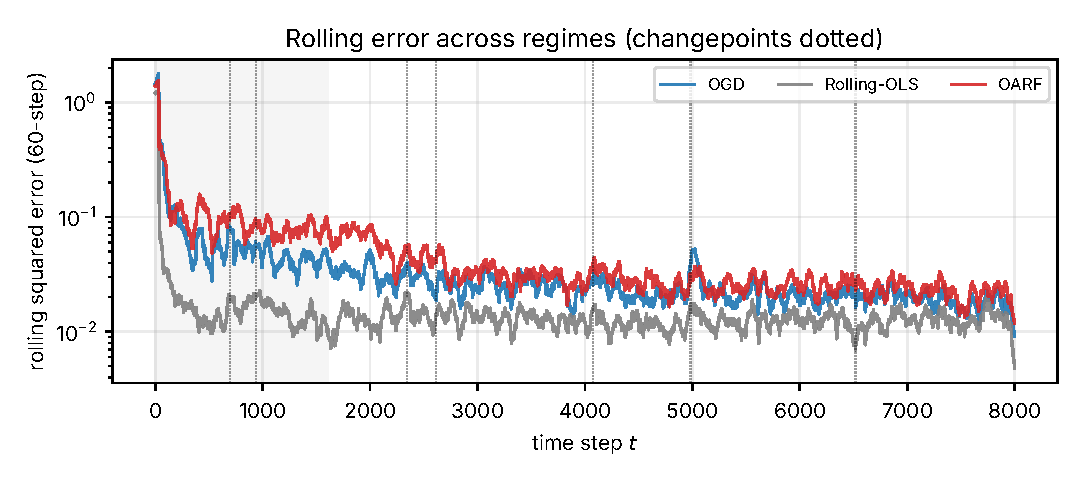
\includegraphics[width=0.86\textwidth]{fig1_rolling_error}
\caption{Rolling squared error across regimes on a representative seed (changepoints
dotted, the shaded band is the warm-up window). The reactive baselines spike at every
break; \OARF{} stays comparatively flat.}
\label{fig:rolling}
\end{figure}

\begin{figure}[htbp]
\centering
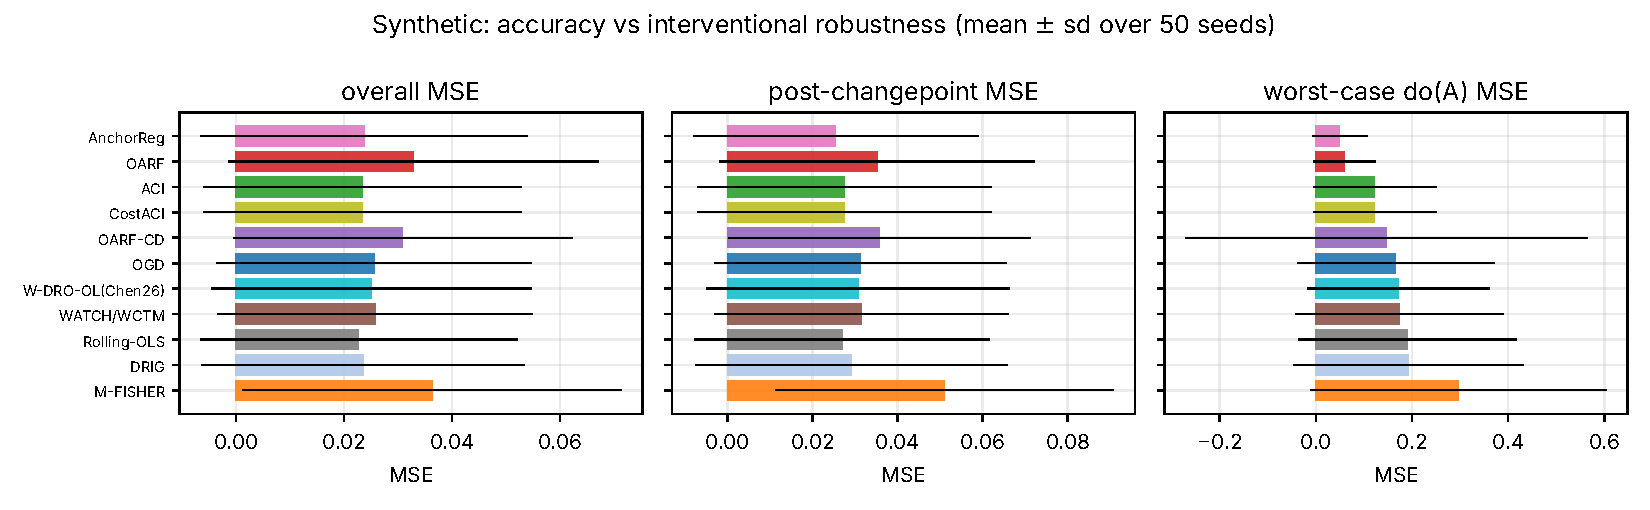
\includegraphics[width=0.92\textwidth]{fig2_bar_metrics}
\caption{Overall, post-changepoint and worst-case interventional MSE on the synthetic
benchmark (means with standard deviations over the $50$ seeds; Table~\ref{tab:syn}
reports medians), sorted by interventional robustness. The reactive and batch methods win in
distribution and \OARF{} and the batch oracle win under intervention, so the two panels are
nearly mirror images.}
\label{fig:bars}
\end{figure}

\begin{figure}[htbp]
\begin{subfigure}{0.5\textwidth}\centering
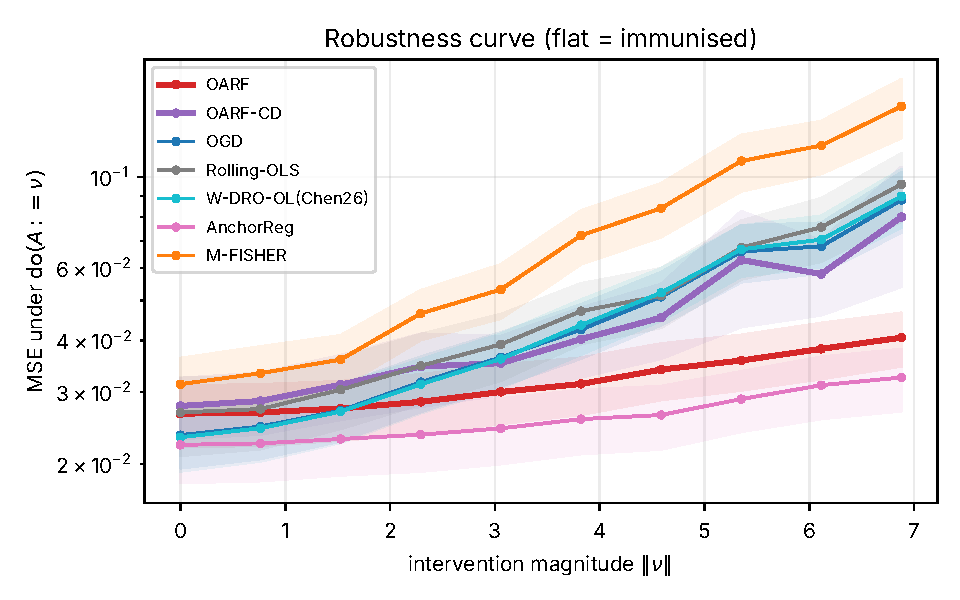
\includegraphics[width=\linewidth]{fig3_robustness_curve}
\caption{Robustness curve: MSE against intervention magnitude $\|\nu\|$.}\label{fig:robust}
\end{subfigure}\hfill
\begin{subfigure}{0.5\textwidth}\centering
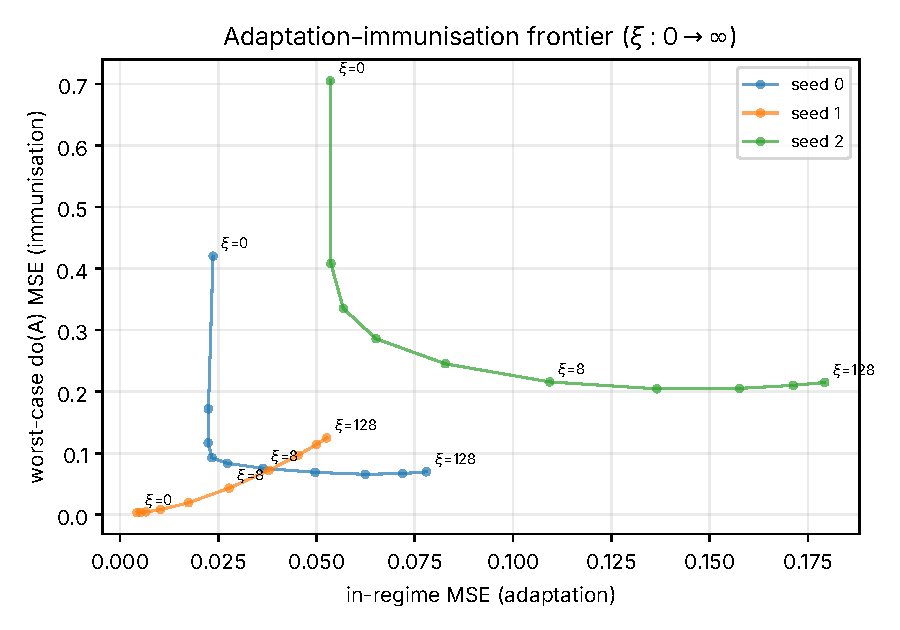
\includegraphics[width=\linewidth]{fig4_pareto}
\caption{Adaptation--robustness frontier as $\xi:0\to\infty$.}\label{fig:pareto}
\end{subfigure}
\caption{(a) \OARF{} and the batch oracle remain near-flat as interventions grow, while
reactive and agnostic-robust methods degrade steeply. (b) The penalty $\xi$ moves the
learner continuously from the online-gradient-descent corner to maximal robustness.}
\label{fig:robust-pareto}
\end{figure}

\begin{figure}[htbp]
\centering
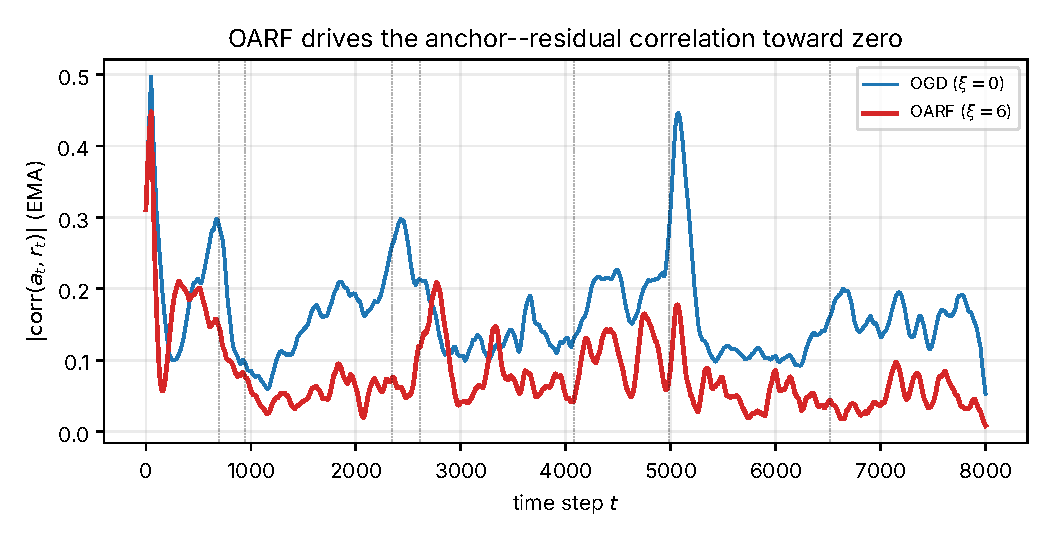
\includegraphics[width=0.78\textwidth]{fig5_immunization}
\caption{Anchor--residual correlation. The smoothed correlation
$|\mathrm{corr}(a_t,r_t)|$ is held near zero by \OARF{} ($\xi=6$) but spikes for online
gradient descent ($\xi=0$) at each regime change (dotted).}
\label{fig:immun}
\end{figure}

\paragraph{Ablations.}
Table~\ref{tab:abl} and Figure~\ref{fig:abl} remove one component at a time. Most of the
interventional robustness comes from the anchor channel. With the true channel the
worst-case interventional error is $0.080$. With a random channel it rises to $0.377$,
which is worse than using no anchor penalty at all (OGD, $0.226$). A wrong channel
therefore does active harm, so identifying the right channel is the main problem; the
stress tests below measure the same effect continuously. The learned channel ($0.303$, alignment $0.84$) is worse than OGD on average in this experiment and, as Section~\ref{sec:learned}
shows, unstable across seeds. AdaGrad matters for both accuracy and robustness: a tuned
fixed step raises in-regime MSE from $0.035$ to $0.095$ and worst-$\doop(A)$ from $0.080$
to $0.145$. EMA centring improves in-regime accuracy ($0.035$ vs.\ $0.043$) with
essentially unchanged robustness, which is consistent with separating the regime mean from
the covariance the penalty uses. For the discovered dimension, worst-$\doop(A)$ MSE and
alignment both improve gradually as $q$ rises from $1$ to $4$ ($0.329\!\to\!0.261$,
alignment $0.79\!\to\!0.90$), because a larger learned subspace still contains the true
two-dimensional channel. Under-specifying the dimension ($q=1$) does more damage, because
the smaller subspace cannot contain it. Results are broadly insensitive to the EMA decay
$\beta$ over $[0.90,0.995]$.

\begin{table}[htbp]
\centering
\caption{Component ablations on the synthetic benchmark (mean over 16 seeds, $\xi=6$
unless noted). The channel carries most of the interventional robustness, and a wrong
channel is worse than none.}
\label{tab:abl}
\small
\begin{tabular}{lcc}
\toprule
Variant & in-regime MSE & worst-$\doop(A)$ MSE\\
\midrule
\OARF{} (full, true channel) & $0.035$ & $\mathbf{0.080}$\\
\quad $-$ EMA centring        & $0.043$ & $0.081$\\
\quad $-$ AdaGrad (fixed step) & $0.095$ & $0.145$\\
\quad random channel          & $0.032$ & $0.377$\\
\quad $\xi=0$ (OGD)           & $0.027$ & $0.226$\\
\midrule
learned channel (\OARFCD{}, alignment $0.84$) & $0.033$ & $0.303$\\
\bottomrule
\end{tabular}
\end{table}

\begin{figure}[htbp]
\centering
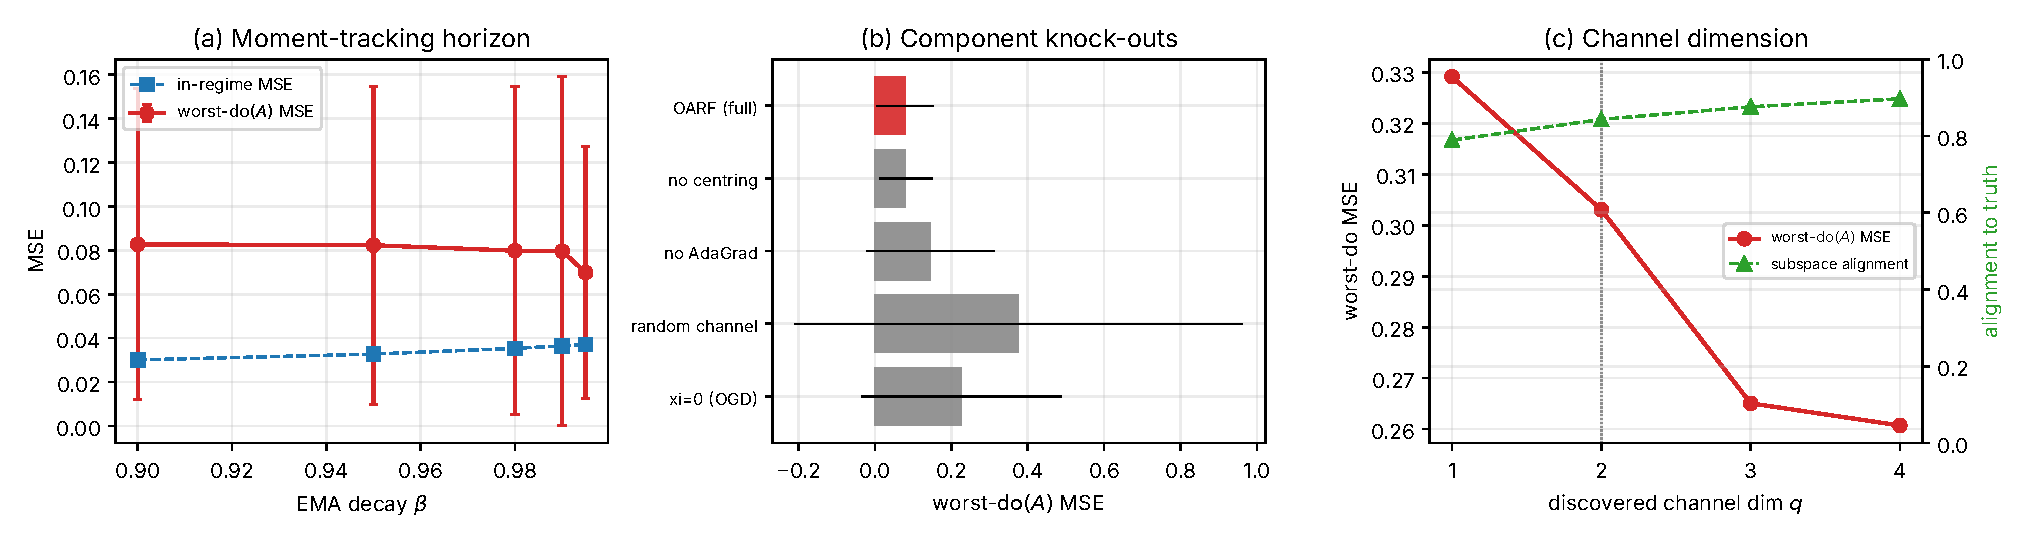
\includegraphics[width=0.99\textwidth]{fig11_ablations}
\caption{Ablations. (a) Sensitivity to the EMA decay $\beta$. (b) Component knock-outs by
worst-case interventional MSE: the channel and the adaptive step matter most, and a
random channel is worse than none. (c) Discovered-channel dimension: robustness and alignment both improve slightly with $q$ (true $q=2$ dotted), but worst-case error stays above OGD at every $q$.}
\label{fig:abl}
\end{figure}

\paragraph{Stress tests.}
The synthetic benchmark favours \OARF{} by construction, because the anchor is clean and
fully observed. In practice it may be neither, so we stress the fixed-channel method
along two axes that break these conditions (Figure~\ref{fig:stress}; the synthetic SCM
is otherwise unchanged, 8 seeds). First, we add noise of growing scale to the observed
context before any method sees it. Worst-$\doop(A)$ MSE rises monotonically with the
noise scale, and \OARF{} crosses the no-anchor OGD baseline at roughly one standard
deviation of observation noise ($0.18$ vs.\ OGD $0.19$). Beyond that point a noisy
anchor is no better than no anchor, and the learned channel degrades sooner. Second, we
rotate the supplied channel away from the truth by an angle $\theta$ (subspace
alignment $\cos\theta$). \OARF{} beats OGD while the alignment exceeds about $0.6$
(roughly $\theta\le 50^\circ$). With a more misaligned channel it is worse than OGD,
reaching $0.36$ against OGD's $0.19$ when the channel is orthogonal; the random-channel
row of Table~\ref{tab:abl} reflects the same mechanism. \OARF{} should therefore be
deployed only when the analyst has reason to believe the anchor is informative, that
is, with alignment well above $0.6$ and noise below order one. A weak or guessed channel can make forecasts worse than using no anchor.

\begin{figure}[htbp]
\centering
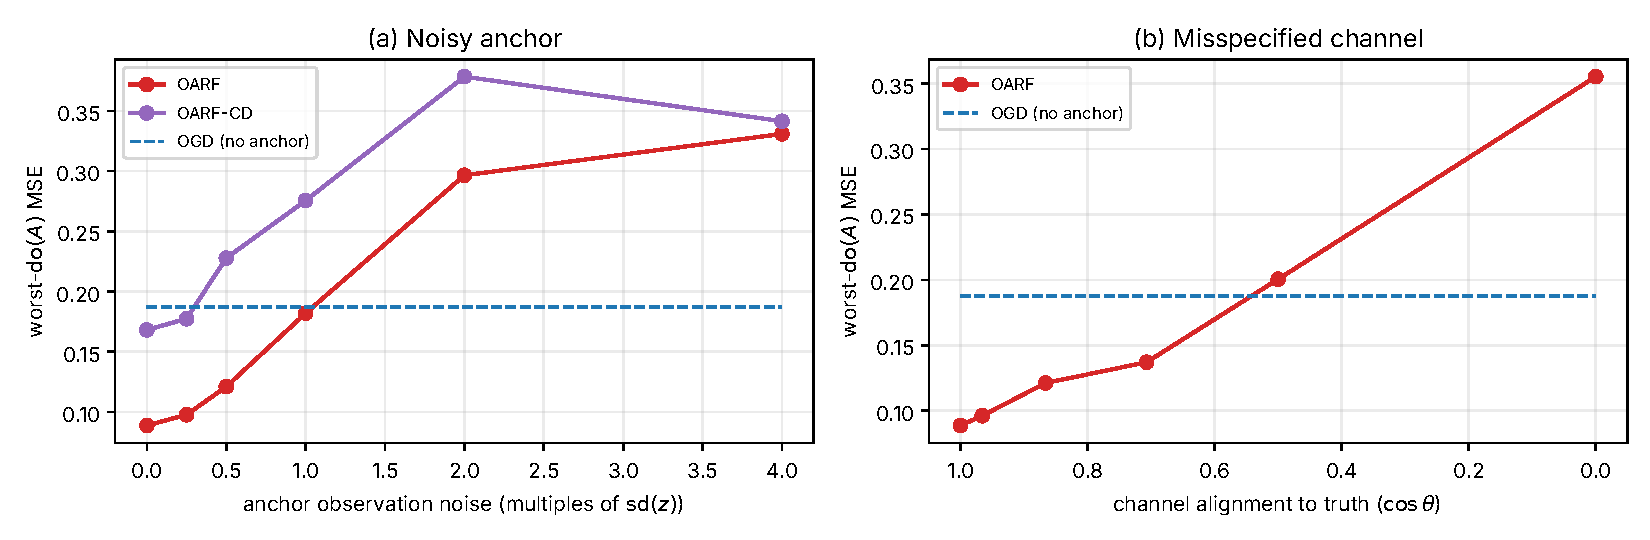
\includegraphics[width=0.97\textwidth]{fig12_stress}
\caption{Stress tests of the fixed-channel method (worst-$\doop(A)$ MSE; OGD baseline
dashed). (a) Increasing anchor observation noise: \OARF{} crosses the no-anchor baseline
near one standard deviation of noise. (b) Rotating the channel away from the truth:
anchoring helps while alignment $\cos\theta\gtrsim 0.6$ and hurts beyond that
point.}
\label{fig:stress}
\end{figure}

\paragraph{Assumption-violation scenarios.}
The stress tests vary the quality of the anchor. We also change the SCM structure so as
to break the assumptions behind Proposition~\ref{prop:equiv} one at a time
(Table~\ref{tab:scen}, median worst-$\doop(A)$ MSE over 8 seeds). \OARF{} keeps its
advantage over OGD in three of these scenarios: when the intervention also shifts the
parents (\textsc{parents}), because the invariant predictor remains valid; when a second
regime driver is unobserved (\textsc{unobserved}), because robustifying the observed
part still helps; and when the observed anchor is a noisy proxy for the true latent
driver (\textsc{proxy}). The method therefore degrades gradually under these
violations. It fails in two cases. When the regime shifts the target's own
parent-coefficient (\textsc{mechanism}), no fixed predictor is robust and both methods
collapse ($\ge\!1.0$). When regimes shift the variance instead of the mean
(\textsc{variance}), the mean-shift equivalence does not apply and \OARF{} is worse than
OGD. The theory covers neither case, and we regard both as limitations of the method.

\begin{table}[htbp]
\centering
\caption{Assumption-violation scenarios (median worst-$\doop(A)$ MSE over 8 seeds;
lower is better). \OARF{} uses the true observed channel. It fails under a shifting
target mechanism and when regimes shift the variance instead of the mean.}
\label{tab:scen}
\small
\begin{tabular}{lcccl}
\toprule
Scenario & \OARF{} & \OARFCD{} & OGD & assumption broken\\
\midrule
clean (ideal)      & $0.021$ & $0.033$ & $0.051$ & none (reference)\\
parents shifted    & $0.018$ & $0.016$ & $0.047$ & none (still anchor-mediated)\\
unobserved driver  & $0.024$ & $0.040$ & $0.048$ & channel incompletely observed\\
noisy proxy anchor & $0.044$ & $0.058$ & $0.065$ & anchor predictive, not causal\\
\midrule
mechanism shift    & $1.299$ & $1.238$ & $1.020$ & target mechanism non-invariant\\
variance shift     & $0.046$ & $0.040$ & $0.025$ & regimes shift variance, not mean\\
\bottomrule
\end{tabular}
\end{table}

\paragraph{Significance.}
On in-distribution loss the Model Confidence Set (computed per seed over $16$ seeds)
retains the batch and conformal methods (Rolling-OLS in all $16$ seeds, DRIG in $15$,
the conformal heads in $11$) and excludes fixed-channel \OARF{} (retained in no seed)
and \OARFCD{} (one seed). This is expected, because \OARF{} gives up in-distribution
accuracy for interventional robustness and in-distribution loss does not reward that.
The Diebold--Mariano statistics on the synthetic benchmark are large
(Figure~\ref{fig:dm}).

\begin{figure}[htbp]
\centering
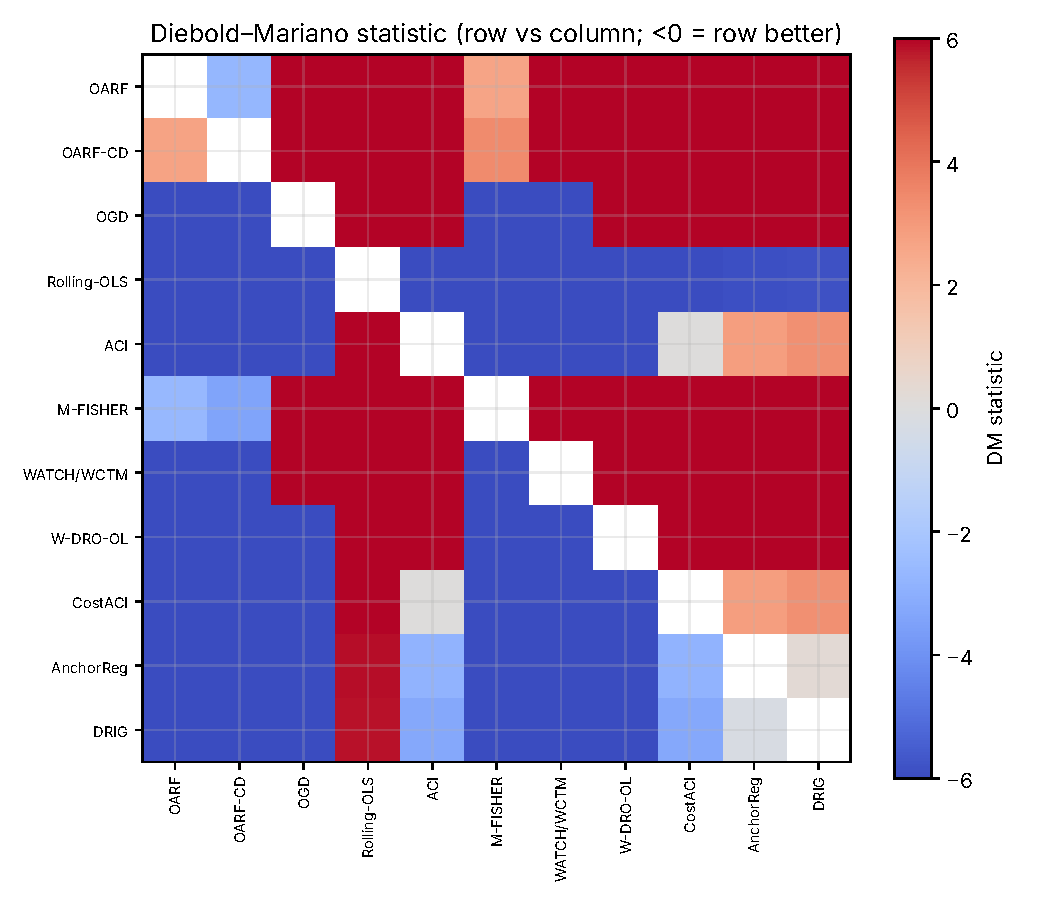
\includegraphics[width=0.62\textwidth]{fig8_dm_heatmap}
\caption{Pairwise Diebold--Mariano statistics on the synthetic benchmark; a negative
entry means the row method is significantly more accurate than the column method.}
\label{fig:dm}
\end{figure}

\section{Weekly energy volatility}\label{sec:real}

The simulation tells us what \OARF{} can do when its assumptions hold. This section
asks whether any of that carries over to a real forecasting problem in which the
assumptions can at best hold approximately.

\paragraph{Data and target.}
We use a public daily panel (Table~\ref{tab:realdata}) aligned to business days with a
forward-fill capped at five days. The targets are the price volatility of Brent crude
and of Henry Hub natural gas. Only daily closing prices are freely available, so
intraday realised variance cannot be formed. We therefore forecast weekly realised
variance from daily returns: for the week ending on Friday $w$, the target is
$y_w=\log\sum_{s\in w}r_s^2$, the log of the sum of squared daily log returns in that
week, and every forecast of $y_w$ uses data up to the end of week $w-1$ only.
Consecutive weeks do not overlap, so no part of the target is known when the forecast
is made. This choice matters. A daily target built from a trailing five-day mean of
squared returns shares four of its five terms with its own lag; on Brent its
correlation with yesterday's value is $0.89$, against $0.53$ for the weekly target, and
most of its apparent predictability is mechanical. Appendix~\ref{app:daily} reports the
daily design for comparison. The sample runs from April 2010 to the week of 26 June
2026 ($847$ weeks); the first $169$ weeks are the warm-up and the remaining $678$
(from July 2013) are evaluated.

\begin{table}[htbp]
\centering
\caption{The public real-data panel. All series are free and are fetched by the
released download script \citep{dang2026oarfcode}; the version used here was
downloaded on 4 November 2026 \citep{fred2026data,caldara2026gprdata,baker2026epudata}.}
\label{tab:realdata}
\small
\begin{tabular}{llll}
\toprule
Series & Source / ticker & Span & Role\\
\midrule
Brent crude & FRED \texttt{DCOILBRENTEU} & 2010--2026 & target\\
Henry Hub gas & FRED \texttt{DHHNGSP} & 2010--2026 & target\\
VIX & FRED \texttt{VIXCLS} & 2010--2026 & driver, anchor\\
EUR/USD & FRED \texttt{DEXUSEU} & 2010--2026 & driver\\
10-year Treasury yield & FRED \texttt{DGS10} & 2010--2026 & driver\\
Geopolitical Risk index & \citet{caldara2022gpr} & 2010--2026 & driver, anchor\\
Economic Policy Uncertainty & \citet{baker2016epu} & 2010--2026 & driver, anchor\\
\bottomrule
\end{tabular}
\end{table}

\paragraph{The anchor and what it assumes.}
The anchor is the end-of-week level of three uncertainty indices: the CBOE VIX, the
daily Geopolitical Risk index and the daily Economic Policy Uncertainty index. The
other drivers (the dollar exchange rate, the ten-year yield, their weekly changes and
lagged volatility) enter the context but not the anchor. For \OARF{} to help, the
regime shifts that matter for energy volatility would have to move the level of these
indices, and the indices would have to behave roughly like the exogenous anchor of
Proposition~\ref{prop:equiv}. The two news-based indices are constructed from
newspaper text and are not computed from energy prices, which makes them the more
plausible candidates. The VIX is a market price that responds to many of the same
shocks as commodity volatility, so it is the least plausible. None of the three is
known to be the channel through which energy-volatility regimes travel. The stress
tests of Section~\ref{sec:synth} tell us what to expect if the anchor is only weakly
aligned with the true channel or observed with noise: little or no gain, and possibly a
small loss. The real study is therefore a test of whether these indices are good
enough anchors, as well as a test of the method.

\paragraph{Forecast pool and benchmarks.}
Every method combines the same seven one-week-ahead forecasts. They are last week's log
realised variance; its means over the previous $4$ and $13$ weeks, in the spirit of the
HAR model \citep{corsi2009har}; a RiskMetrics exponentially weighted variance and a
GARCH$(1,1)$ variance, both computed from daily returns up to the end of the previous
week and scaled to five days; the log VIX at the end of the previous week; and a
rolling ridge regression on five lags of the target and the lagged drivers, whose
features are standardised with the statistics of its own training window. The methods
are \OARF{}, \OARFCD{} and nine of the baselines of Table~\ref{tab:baselines}
(WATCH/WCTM, CostACI and DRIG are not run on the real data), with the hyper-parameters
of Table~\ref{tab:hyper}; nothing was re-tuned for the weekly data. We add two fixed
benchmarks that a forecasting reader would expect: persistence, which forecasts this
week's log variance by last week's, and the equal-weight average of the six members of
the pool that forecast log variance directly (the log VIX is on a different scale and
is left out). Both benchmarks are scored under the same protocol as the learning
methods. Regimes for the regime-aware metrics are terciles of the lagged four-week mean
of the target, with segments shorter than eight weeks merged into their neighbours.
The tercile thresholds use the full sample; the labels are used only to score
forecasts and no method sees them.

\paragraph{Results.}
Table~\ref{tab:real} reports the results, and Figure~\ref{fig:real} shows the Brent
error path. The first finding is that the combination methods are useful. On both
series every learned combination has a lower MSE than persistence; for most methods
the reduction is about a third on Brent and a fifth on Henry Hub. On Brent the Model Confidence Set excludes
persistence ($p<0.01$) and the expected-shortfall combiner ($p=0.06$) and retains the
other eleven methods. On Henry Hub it retains all thirteen, persistence included
($p=0.17$), so the gain over persistence there is not significant at the $10\%$ level.

The second finding is that \OARF{} adds nothing on these data. Its MSE is within $1.5\%$
of online gradient descent on both series (Brent $0.714$ against $0.704$, Henry Hub
$1.014$ against $1.009$), it is slightly worse in the worst regime, and the
equal-weight average does as well as either. The batch anchor-regression reference does
best on Henry Hub ($0.984$) and among the worst on Brent ($0.741$). None of these
differences is significant. Apart from persistence on Henry Hub ($0.17$) and anchor
regression on Brent ($0.52$), every retained method has an MCS $p$-value of $1.00$. The
pairwise Diebold--Mariano test of \OARF{} against online gradient descent gives
$p=0.47$ on Brent and $p=0.54$ on Henry Hub (Figure~\ref{fig:real-dm}). Some pairs of
baselines do differ in the pairwise test, for example ACI and W-DRO-OL on Brent, but
the Model Confidence Set, which accounts for the number of comparisons, keeps them
together. The coverage of the conformal head is $0.86$ on Brent
and $0.87$ on Henry Hub, against a nominal $0.90$.

This is the outcome the stress tests predict if the uncertainty indices are noisy or
weakly aligned proxies for whatever moves energy volatility, and the data do not let us
separate that explanation from the alternative that energy-volatility regimes are not
anchor-mediated mean shifts at all. Two secondary checks give the same picture. A
volatility-timing strategy built on each forecast earns low Sharpe ratios whose ranking
does not follow forecast accuracy (Appendix~\ref{app:econ}). In two event windows,
the COVID-19 crash of 2020 and the energy shock of 2022, \OARF{} has a lower
cumulative loss than online gradient descent in three of the four window--commodity
pairs and a higher one in the fourth, the 2022 window for Brent
(Appendix~\ref{app:events}).

\begin{table}[htbp]
\centering
\caption{Weekly log realised variance, non-overlapping weeks, evaluation over the last $678$ of $847$ weeks (2013--2026). MSE is on the target's past-only standardised scale, so persistence and the learned combinations are directly comparable; w-reg is the worst-regime MSE and post-cp the MSE in the $50$ weeks after each regime change. MCS $p$ is the Model Confidence Set $p$-value \citep{hansen2011mcs}; methods with $p<0.10$ are outside the $10\%$ set. The two fixed benchmarks are listed first.}
\label{tab:real}
\small
\setlength{\tabcolsep}{4pt}
\resizebox{\linewidth}{!}{%
\begin{tabular}{lcccc|cccc}
\toprule
& \multicolumn{4}{c|}{Brent} & \multicolumn{4}{c}{Henry Hub}\\
Method & MSE & w-reg & post-cp & MCS $p$ & MSE & w-reg & post-cp & MCS $p$\\
\midrule
Persistence & $1.072$ & $1.306$ & $1.025$ & $<0.01$ & $1.267$ & $1.664$ & $1.448$ & 0.17\\
Equal-weight average & $0.708$ & $0.802$ & $0.687$ & 1.00 & $1.013$ & $1.269$ & $1.107$ & 1.00\\
\midrule
\textbf{\OARF{}} & $0.714$ & $0.823$ & $0.689$ & 1.00 & $1.014$ & $1.287$ & $1.124$ & 1.00\\
\OARFCD{} (Section~\ref{sec:learned}) & $0.713$ & $0.800$ & $0.710$ & 1.00 & $0.987$ & $1.264$ & $1.108$ & 1.00\\
OGD & $0.704$ & $0.804$ & $0.687$ & 1.00 & $1.009$ & $1.261$ & $1.129$ & 1.00\\
Rolling-OLS & $0.712$ & $0.826$ & $0.685$ & 1.00 & $1.047$ & $1.301$ & $1.208$ & 1.00\\
ACI & $0.720$ & $0.831$ & $0.697$ & 1.00 & $0.995$ & $1.256$ & $1.106$ & 1.00\\
M-FISHER (2025) & $0.730$ & $0.856$ & $0.715$ & 1.00 & $1.110$ & $1.311$ & $1.227$ & 1.00\\
DR-Combo (Wang 2026) & $0.723$ & $0.815$ & $0.714$ & 1.00 & $1.054$ & $1.302$ & $1.184$ & 1.00\\
FC-DRO (Liu 2026) & $0.713$ & $0.800$ & $0.696$ & 1.00 & $1.088$ & $1.276$ & $1.177$ & 1.00\\
FC-DRO-ES (Liu 2026) & $0.898$ & $0.985$ & $0.847$ & 0.06 & $1.134$ & $1.503$ & $1.299$ & 1.00\\
W-DRO-OL (Chen 2026) & $0.704$ & $0.804$ & $0.687$ & 1.00 & $1.010$ & $1.263$ & $1.129$ & 1.00\\
AnchorReg (rolling batch) & $0.741$ & $0.844$ & $0.706$ & 0.52 & $0.984$ & $1.230$ & $1.125$ & 1.00\\
\bottomrule
\end{tabular}}
\end{table}

\begin{figure}[htbp]
\centering
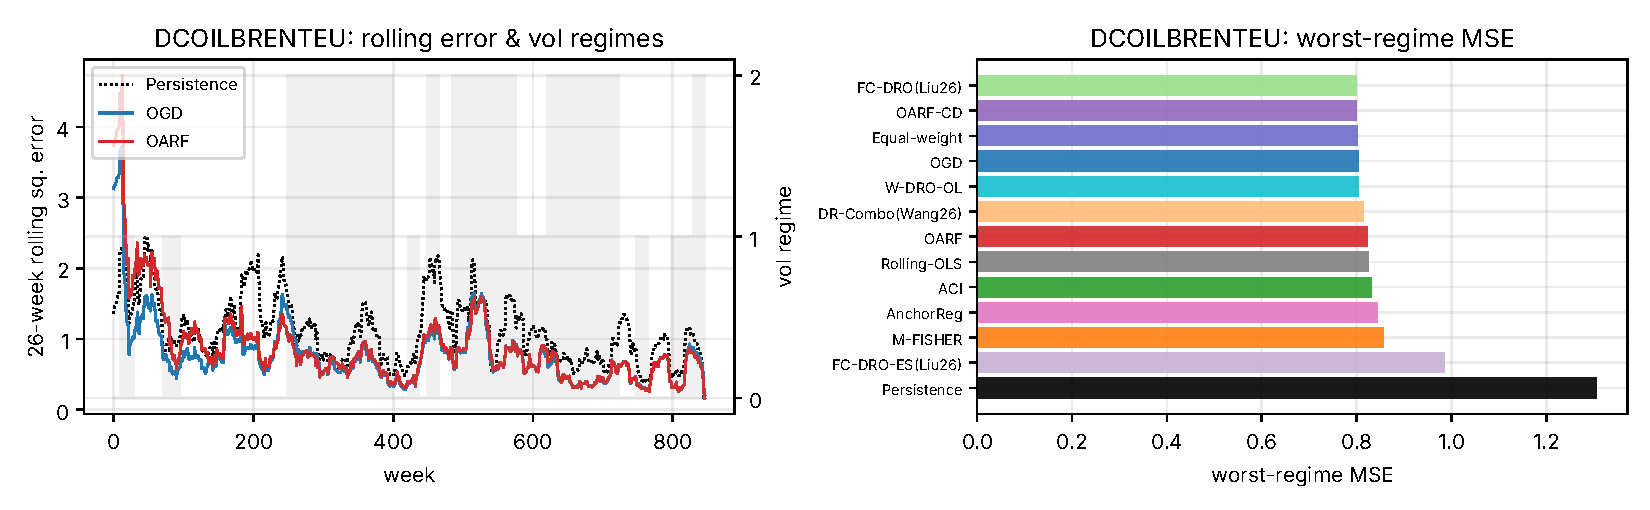
\includegraphics[width=0.97\textwidth]{fig9_real_DCOILBRENTEU}
\caption{Brent, weekly design. Left: $26$-week rolling squared error of persistence,
OGD and \OARF{}, with the volatility regime shaded. Right: worst-regime MSE by method.}
\label{fig:real}
\end{figure}

\begin{figure}[htbp]
\centering
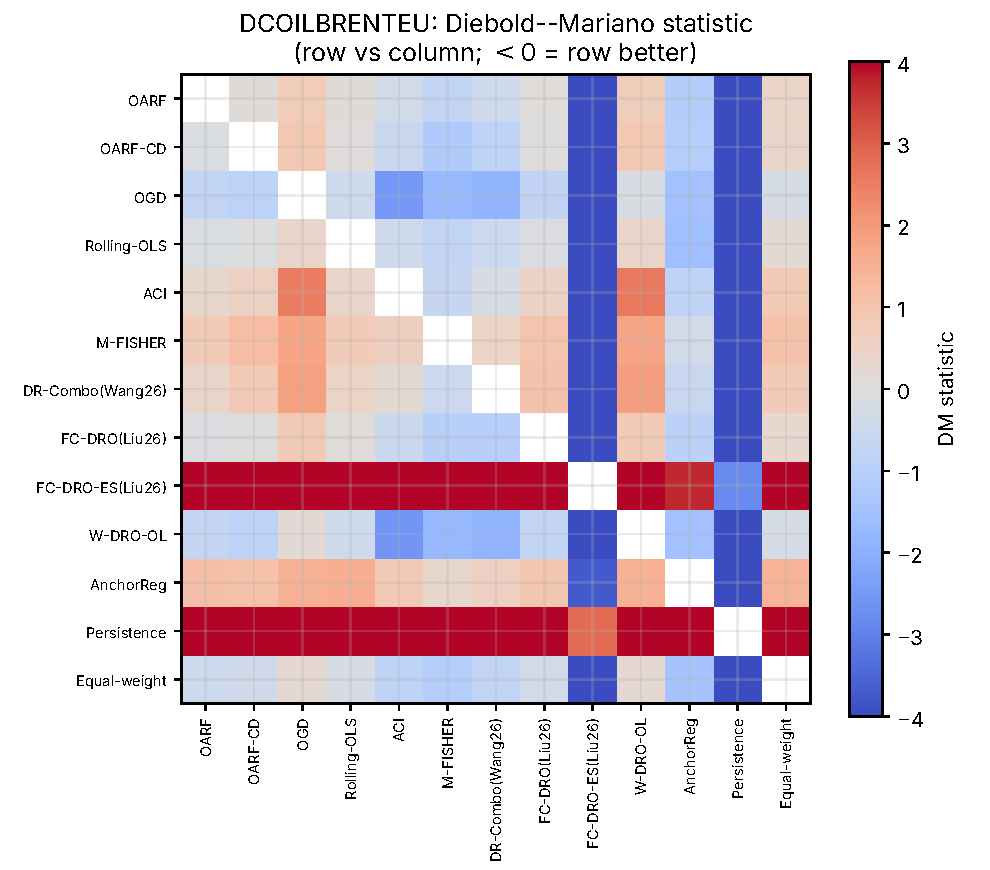
\includegraphics[width=0.62\textwidth]{fig13_dm_DCOILBRENTEU}
\caption{Brent, weekly design: pairwise Diebold--Mariano statistics (negative means the
row method is more accurate than the column method). Persistence and the
expected-shortfall combiner are clearly worse than the rest; among the other methods
most statistics are small.}
\label{fig:real-dm}
\end{figure}

\section{Extension: learning the anchor}\label{sec:learned}

So far the analyst has supplied the anchor. In practice the channel is often
uncertain: Section~\ref{sec:real} used three candidate indices without knowing whether
any of them carries the regime. This section describes a rule, \OARFCD{}, that
estimates the channel from the stream, a statistic that indicates when the estimate can
be trusted, and the evidence on both. Theorem~\ref{thm:main} does not cover the learned
channel.

\subsection{Method}

\paragraph{Online channel discovery.}
The rule estimates $B$ from the stream. It performs unsupervised nonstationary-subspace estimation, not causal discovery. Under the SCM of
Proposition~\ref{prop:equiv}, a regime acts on the context by shifting the anchor's
location, so the anchor directions are nonstationary in mean across regimes and
stationary nuisance directions are not. We therefore track the across-regime
dispersion of the context's conditional mean and ascend it on a slow timescale
$\eta_B\ll\eta$,
\begin{equation}\label{eq:channel}
\max_{\|B\|_F\le 1}\ \mathcal{D}(B)=\Var_{\text{regimes}}\!\big(\E[B^\top z\mid\text{regime}]\big)
 -\gamma_c\,\big\|\E[B^\top z]\big\|^2 .
\end{equation}
This objective selects high-dispersion nonstationary directions. It does not by itself
establish that they are exogenous or causal. The grand-mean penalty (second term)
discourages loading on the persistent component but does not guarantee exogeneity,
and a direction that is only volatile or trending can be selected; the stress tests of
Section~\ref{sec:synth} probe this failure mode. What the layer recovers is the
subspace through which regimes appear to act in the observable context, and this
coincides with the causal channel only under the SCM assumptions.

Streaming \eqref{eq:channel} needs a proxy for ``regime''. We use a forgetting
partition into length-$L$ blocks. A block should be long enough for a stationary
driver's short-horizon autocorrelation to average out within it (so $L$ should exceed
the dominant driver autocorrelation time), and short enough that actual regime changes
fall across block boundaries. The block length $L$ is a hyperparameter selected on the warm-up window. Let $S$ be
the across-block scatter of the block-mean context and $u$ its grand mean. The ascent
direction is $\nabla_B\mathcal{D}=2(S-\gamma_c uu^\top)B$. At each block boundary $B$
is updated after that step's robust gradient step and re-orthonormalised onto the
Frobenius ball, and the new $B$ is used from the next step onward. A lightweight
non-robust reference predictor is run alongside to keep discovery oriented toward
predictively relevant directions. Algorithm~\ref{alg:oarf} gives the complete loop,
with discovery as an optional inner block.

\paragraph{Reliability diagnostic.} The discovery layer can fail silently. Nothing in
Algorithm~\ref{alg:oarf} tells the forecaster whether the current $B$ is a good
estimate of the true channel, and in deployment the true channel is unobserved. As a
proxy for how well the top-$q$ subspace is identified, we use a quantity the layer
already computes. Let $\lambda_1\ge\cdots\ge\lambda_p$ be the eigenvalues of
$M=S-\gamma_c uu^\top$ at a given block boundary (Eq.~\eqref{eq:channel}), and define
the \emph{normalised eigengap}
\begin{equation}\label{eq:eigengap}
 \kappa \;=\; \frac{\lambda_q-\lambda_{q+1}}{\sum_{i=1}^p|\lambda_i|+\epsilon}\in[0,1].
\end{equation}
By the Davis--Kahan $\sin\Theta$ theorem, the angle between the top-$q$ eigenspace of
an estimated symmetric matrix and that of the population matrix it estimates is
controlled by the corresponding population eigengap. A small $\kappa$ means that the $q$-dimensional subspace $B$ is ascending is only weakly separated from
the rest of the spectrum, so which $q$ directions are selected depends on sampling
noise. A large $\kappa$ means the top-$q$ subspace is well separated and stably
identified. The subspace alignment used below to score the discovery layer against ground
truth needs the true channel, whereas $\kappa$ is
computed entirely from the stream and is available in a live deployment.
Davis--Kahan bounds estimation error given a population gap; it says nothing about
whether the recovered subspace is exogenous or causal, which still rests on the SCM
assumptions of Proposition~\ref{prop:equiv}. The evidence below tests whether
$\kappa$ tracks true recovery and whether gating on it helps.

\subsection{Evidence}

\paragraph{Learned channel.}
When it has to find its own anchor, \OARFCD{} recovers the true subspace on average. Mean
principal-subspace alignment is $0.88\pm0.16$, against a random-subspace baseline of
$0.42$, and individual seeds climb toward $0.99$ as the stream lengthens
(Figure~\ref{fig:channel}). Its median worst-$\doop(A)$ MSE ($0.049$) is close to that of
fixed-channel \OARF{} ($0.041$, Table~\ref{tab:syn}), but the distribution has a heavy
tail. The mean across seeds is $0.147$, roughly three times the median, and on a minority
of seeds the error approaches or exceeds that of OGD (median $0.095$), which applies no
anchor penalty. A seed's final alignment is only noisily related to its worst-$\doop(A)$
MSE (Figure~\ref{fig:scatter}), and the seeds with poor alignment account for the tail.
The layer therefore recovers a nonstationary subspace but does not match the
robustness of a known channel, and this tail is its main practical limitation.

\begin{figure}[htbp]
\centering
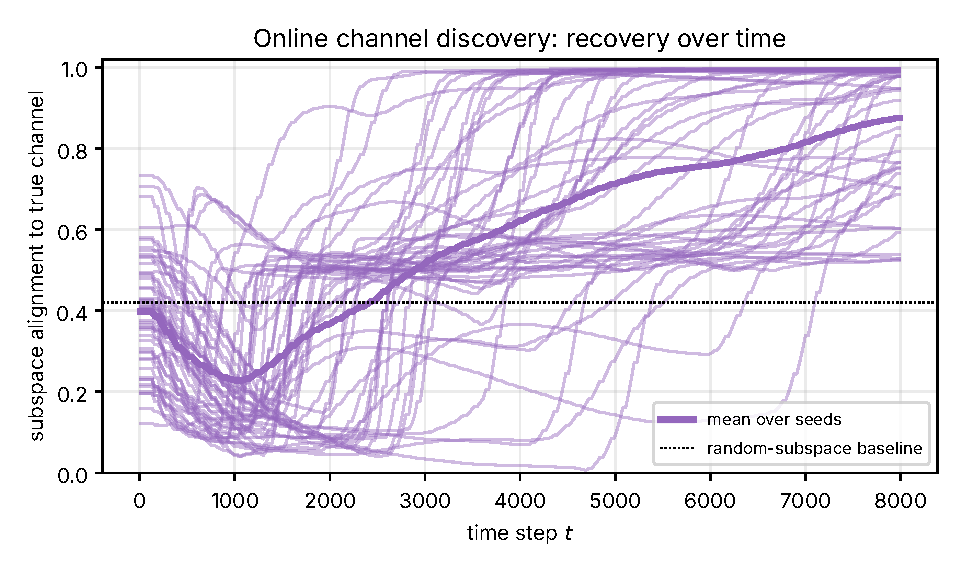
\includegraphics[width=0.72\textwidth]{fig6_learned_channel}
\caption{Online channel discovery: alignment of the learned channel $B_t$ to the true
intervention subspace over time. Thin lines are individual seeds, the bold line is their
mean, and the dotted line is the random-subspace baseline.}
\label{fig:channel}
\end{figure}

\begin{figure}[htbp]
\centering
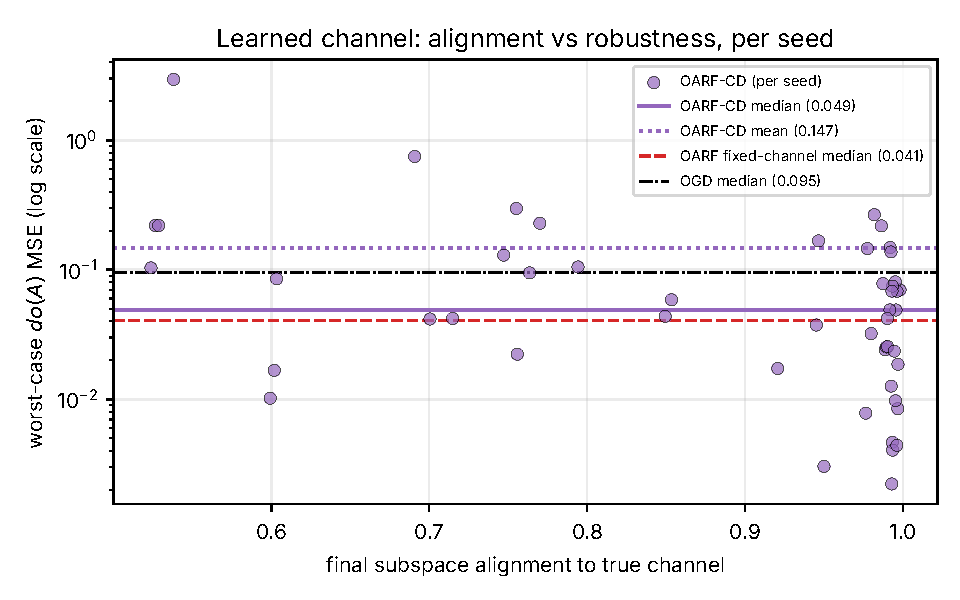
\includegraphics[width=0.74\textwidth]{fig14_alignment_scatter}
\caption{Per-seed alignment versus interventional robustness for the learned channel
($50$ seeds). Each point is one seed: the horizontal axis is the final subspace
alignment of \OARFCD{}'s discovered channel and the vertical axis its worst-case
$\doop(A)$ MSE (log scale). High-alignment seeds cluster at low error near the
fixed-channel \OARF{} median (dashed), but a minority of low-alignment seeds incur an
order-of-magnitude higher error. These seeds pull the mean (dotted) far above the median
(solid) and make the learned channel unreliable in the worst case.}
\label{fig:scatter}
\end{figure}

\paragraph{Online reliability diagnostic.}
Figure~\ref{fig:scatter} shows that the failures of the discovery layer are a discrete tail
risk. Most seeds recover a well-aligned channel, a minority do not, and those seeds dominate
the mean worst-case error. If they could be flagged while the stream runs, without
consulting the true channel (which a deployment never observes), the layer could decline to
trust its own channel on those streams. Figure~\ref{fig:diagnostic}a tests whether the
eigengap $\kappa$ of Eq.~\eqref{eq:eigengap} can serve as such a flag. Across the $50$
seeds, $\kappa$ correlates with the true subspace alignment, which is otherwise
unobservable, at $r=0.62$, and $13$ of the $16$ seeds whose final alignment falls below
$0.8$ also fall in the bottom quartile of post-warm-up eigengap. Figure~\ref{fig:diagnostic}b
uses this as a gate. When a seed's average post-warm-up $\kappa$ lies in the bottom
quartile (only~$13$ of $50$ seeds), the forecaster reverts to plain OGD; otherwise it
keeps the learned channel. Gating lowers the mean worst-$\doop(A)$ MSE of \OARFCD{} from
$0.147$ (ungated) to $0.113$, a reduction of about a quarter, and closes about two-fifths
of the gap to the $0.059$ attained with the true channel. The gate uses only a statistic the discovery layer already computes. Its threshold, however, is the
$25$th percentile of $\kappa$ across these same $50$ seeds, so in deployment it would
have to be calibrated in advance, for example on simulated streams. The decision uses
the average of $\kappa$ over the second half of each stream, so the gate makes one choice per stream. It also discards a misspecified channel
instead of correcting it; like Davis--Kahan, a large gap certifies a well-identified
subspace but says nothing about whether that subspace is exogenous.

\begin{figure}[htbp]
\centering
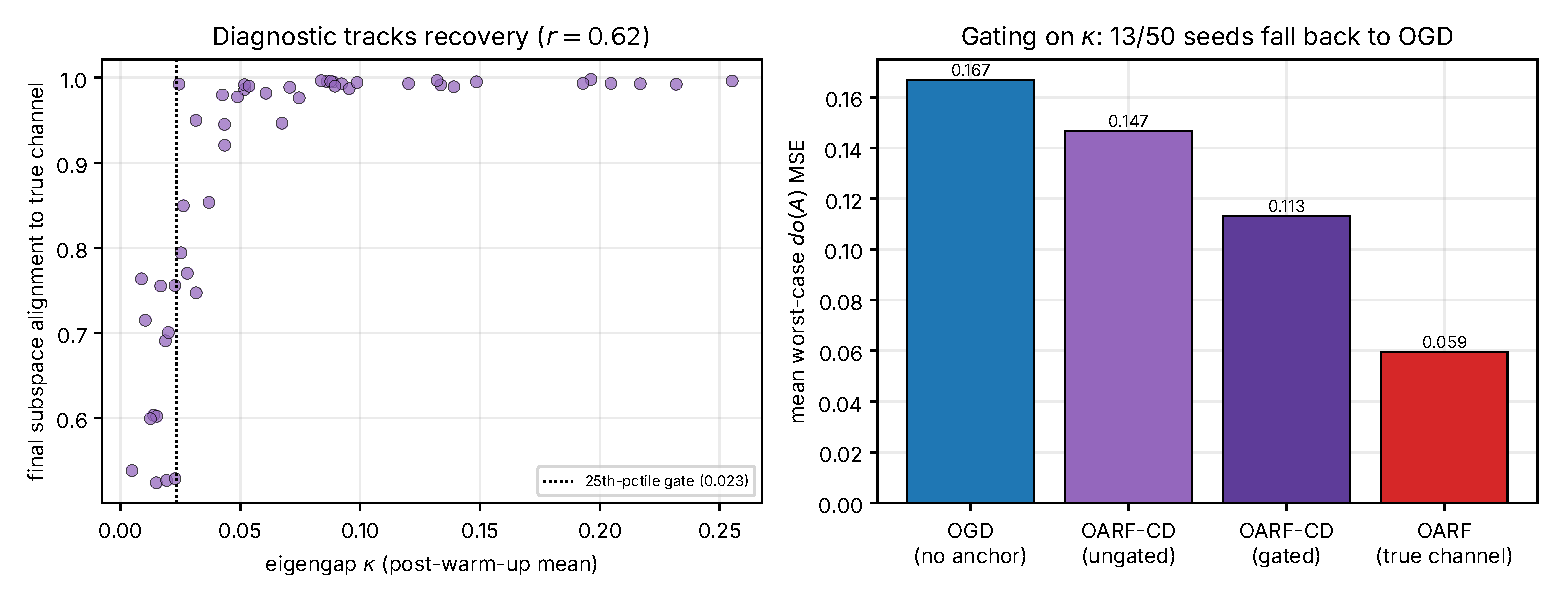
\includegraphics[width=0.98\textwidth]{fig16_eigengap_diagnostic}
\caption{Eigengap diagnostic. (a) Per-seed post-warm-up eigengap
$\kappa$ vs.\ true subspace alignment ($r=0.62$); the dotted line is the
$25$th-percentile gate. (b) Mean worst-case $\doop(A)$ MSE for OGD, ungated
\OARFCD{}, \OARFCD{} gated on $\kappa$, and fixed-channel \OARF{} with the true
channel. Gating reduces the ungated learned channel's mean worst-case error by about a
quarter without using the ground truth.}
\label{fig:diagnostic}
\end{figure}

\paragraph{Comparison of anchor selectors.}
Automatic anchor selection is the most fragile part of the method, so we compare the
block-mean rule of OARF-CD with alternative selectors under a strict pre-deployment
budget: the channel is estimated on the warm-up block only, with no look-ahead
(Table~\ref{tab:sel}). The alternatives are a supervised residual--context-coupling
selector, stationary PCA of the context, and a random channel. Each is scored by its
alignment to the truth and by the worst-$\doop(A)$ MSE of the resulting fixed-channel
method. The block-mean rule does about as well as the supervised selector and much better than stationary PCA. From a short warm-up, though, neither is clearly better than a random channel: their worst-$\doop(A)$ MSEs are $0.101$ and $0.093$ against $0.115$ for a random channel and $0.070$ for the true one, and their alignments ($0.42$ and $0.37$) are no higher than the random channel's ($0.43$). High alignment is reached only by learning over the full stream (\OARFCD{}, alignment $0.84$ in Table~\ref{tab:abl}), and even then the estimate is unstable.
Reliable online anchor discovery from limited data thus remains an open problem.
Practitioners should supply a candidate anchor and validate it with the procedure
of Section~\ref{sec:discussion} instead of relying on automatic discovery alone.

\begin{table}[htbp]
\centering
\caption{Anchor selectors estimated on the warm-up block only (8 seeds; alignment to
the true channel, and worst-$\doop(A)$ MSE of the resulting fixed-channel \OARF{};
lower MSE / higher alignment better).}
\label{tab:sel}
\small
\begin{tabular}{lcc}
\toprule
Selector & subspace alignment & worst-$\doop(A)$ MSE (median)\\
\midrule
true channel (reference)             & $1.00$ & $0.070$\\
block-mean (OARF-CD rule)            & $0.42$ & $0.101$\\
supervised residual--context coupling & $0.37$ & $0.093$\\
stationary PCA of context            & $0.31$ & $0.236$\\
random channel                       & $0.43$ & $0.115$\\
\bottomrule
\end{tabular}
\end{table}

\paragraph{Real data.}
On the energy data the learned channel does about as well as the hand-chosen one
(Table~\ref{tab:real}: MSE $0.713$ against $0.714$ on Brent and $0.987$ against
$1.014$ on Henry Hub), and both are inside the Model Confidence Set. Since neither
improves on online gradient descent, these numbers say nothing about whether the
learned channel is closer to the true one.

\section{Discussion and conclusion}\label{sec:discussion}

When a regime shift moves an observed anchor and the forecasting relation is
confounded through that anchor, a forecaster can be made robust to the shift in
advance and online. In our simulation the gain is large: \OARF{} more than halves the
worst-case error of online gradient descent, and it pays for this with a higher
in-distribution error that the penalty $\xi$ controls. Distributionally robust methods
spread their protection over all directions, while anchoring concentrates it on the
directions in which the anchor moves. This helps only if those directions are the right
ones. With an anchor observed with noise of about one standard deviation, or misaligned
with the true channel by more than about $50^\circ$, the benefit is gone, and when
regimes shift variances or the target equation the method does worse than no anchor.

The energy application shows how far this carries to real data. With a target that
does not overlap its own lag, the learned combinations beat persistence, but \OARF{}
with macro-uncertainty indices as the anchor is no better than online gradient descent
or an equal-weight average. We read this as evidence that these indices are, at best,
noisy and weakly aligned proxies for whatever moves energy volatility, which is the
case in which our stress tests predict no gain; the data cannot rule out that energy
regimes are simply not anchor-mediated mean shifts. The earlier daily design, whose
target overlapped its lag, made all methods look more accurate than they are and could
not separate them from persistence (Appendix~\ref{app:daily}).

\paragraph{Using the method.}
These results suggest a simple procedure. Propose candidate anchors from domain
knowledge. On the warm-up block, check that the correlation between the anchor and the
residual of a plain online learner is non-trivial and stable, and run a stress test
that perturbs the anchor as in Figure~\ref{fig:stress}. Use fixed-channel \OARF{} only
if anchoring improves the validation worst-regime loss at an acceptable in-distribution
cost and a random or noisy version of the anchor does not do as well. Otherwise use
plain online learning. Treat a learned channel as a diagnostic unless its eigengap is
large, and do not use the method when the regime shifts appear as changes in variance
or in the target equation.

\paragraph{Limitations.}
The theorem covers the fixed channel with an Ader step wrapper, while the experiments
use AdaGrad (Appendix~\ref{app:ader}), and its $T^{2/3}$ rate for estimated moments
relies on stationarity within regimes. Tightening this rate toward $\sqrt{T}$ without a
changepoint trigger, and extending a guarantee to a learned or misspecified channel,
remain open; the Davis--Kahan bound behind the eigengap check supplies only the
estimation half of such an argument. The real study has $678$ evaluation weeks, uses a
variance proxy from daily closing prices because intraday data are not freely
available, and uses an equity-market implied volatility in the absence of a free
commodity-specific one. Other extensions are nonlinear anchors and predictors and
richer interventions on variances and mechanisms.

\paragraph{Reproducibility.}
All code and data-build scripts that regenerate every number, table and figure in this
paper are available at
\url{https://github.com/vinhqdang/OARF-Online-Anchor-Robust-Forecasting-under-Economic-Regime-Shift}.

\appendix

\section{Proof of Theorem~\ref{thm:main}}\label{app:proof}
Throughout, $\mathcal{R}_t(w):=\sup_{\|\nu\|\le\rho(\xi)}\E_{\doop(a:=\nu)}
[(y_t-w^\top\phi(x_t))^2]$ is the per-step worst-case risk in \eqref{eq:intreg}, and
$\hat g_t$ is the (inexact) step direction of Algorithm~\ref{alg:oarf}.

\begin{lemma}[Convex surrogate and gradient decomposition]\label{lem:surrogate}
$\mathcal{R}_t$ is convex, and under Assumption~\ref{ass:scm} it equals, within the active
regime, the anchor-penalised risk $\mathcal{R}_t(w)=\E_t[(y-w^\top\phi)^2]+\xi P_t(w)$ of
\eqref{eq:bar}. Also, $\hat g_t=\nabla\mathcal{R}_t(w_t)+\zeta_t$ with $\zeta_t=M_t+b_t$,
where $M_t:=-r_t\phi(x_t)-\E_t[-r\phi]$ is a martingale difference
($\E[M_t\mid\mathcal F_{t-1}]=0$) and $b_t$ is the deterministic
($\mathcal F_{t-1}$-measurable) error of the EMA-estimated penalty gradient relative to
$\nabla(\xi P_t)$.
\end{lemma}
\begin{proof}
For fixed $\nu$, $\E_{\doop(a:=\nu)}[(y-w^\top\phi)^2]$ is a convex quadratic in $w$; a
pointwise supremum of convex functions is convex. The identity is
Proposition~\ref{prop:equiv} within the stationary active regime. The prediction term
$-r_t\phi(x_t)$ is an unbiased one-sample estimate of
$\tfrac12\nabla\E_t[(y-w^\top\phi)^2]=-\E_t[r\phi]$, with centred part $M_t$; the
robustness term substitutes the $\mathcal F_{t-1}$-measurable EMA moments for the
population moments in $\nabla(\xi P_t)$, and $b_t$ is that substitution error.
\end{proof}

\begin{lemma}[Inexact dynamic regret]\label{lem:ogd}
Run projected OGD with the path-length-adaptive Ader wrapper
\citep{zhang2018adaptive} on the convex losses $\mathcal{R}_t$, fed $\hat g_t$. Then for any
$u_{1:T}\subset\mathcal{W}$ of path length $P_T$,
$\sum_t\mathcal{R}_t(w_t)-\sum_t\mathcal{R}_t(u_t)\le O(\sqrt{T(1+P_T)})+\sum_t\langle\zeta_t,
w_t-u_t\rangle$, with the first term attained without prior knowledge of $P_T$.
\end{lemma}
\begin{proof}
With exact gradients, Ader attains minimax dynamic regret $O(\sqrt{T(1+P_T)})$ for
convex $G$-Lipschitz losses over a radius-$D$ set, adaptively in $P_T$
\citep{zhang2018adaptive}, subsuming \citet{zinkevich2003ogd,hazan2016oco}. Convexity
gives $\mathcal{R}_t(w_t)-\mathcal{R}_t(u_t)\le\langle\nabla\mathcal{R}_t(w_t),w_t-u_t\rangle=
\langle\hat g_t,w_t-u_t\rangle-\langle\zeta_t,w_t-u_t\rangle$; summing and applying the
exact-gradient bound to the $\hat g_t$ terms yields the inexactness term.
\end{proof}

\begin{lemma}[Gradient-error control]\label{lem:mom}
Under Assumptions~\ref{ass:bounded}--\ref{ass:moment}, against the deterministic
minimising comparator: (i) $\E[\sum_t\langle M_t,w_t-u_t\rangle]=0$; and (ii)
$\E\|b_t\|\le c_1\sqrt{1-\beta}$ at steps at least $1/(1-\beta)$ into a regime, with
$\|b_t\|\le c_2$ within $1/(1-\beta)$ steps of each of the $K$ changes, so
$\sum_t\E\|b_t\|\le c_1 T\sqrt{1-\beta}+c_2 K/(1-\beta)$; with oracle moments $b_t\equiv0$.
\end{lemma}
\begin{proof}
(i) $w_t$ is $\mathcal F_{t-1}$-measurable and, the schedule being oblivious
(Assumption~\ref{ass:comp}), $u_t$ is deterministic, so
$\E[\langle M_t,w_t-u_t\rangle\mid\mathcal F_{t-1}]=0$; the tower rule concludes. (ii) An
EMA of decay $\beta$ of a stationary sequence has variance $\Theta(1-\beta)$ about its
mean and geometrically-decaying within-regime bias; by Assumption~\ref{ass:bounded} the
penalty gradient is Lipschitz in these moments (the $\epsilon$-ridge bounds the
inverse), inheriting the $\Theta(\sqrt{1-\beta})$ steady-state scale. After a change the
EMA mixes the previous regime for $O(1/(1-\beta))$ steps with bounded $\|b_t\|\le c_2$.
Summing gives the bound; oracle moments make the substitution error vanish.
\end{proof}

\begin{proof}[Proof of Theorem~\ref{thm:main}]
Combining the lemmas and taking expectations, for the deterministic minimiser
$u_{1:T}\in\mathcal{W}$ ($P_T\le 2DK$),
$\E[\sum_t\mathcal{R}_t(w_t)]-\sum_t\mathcal{R}_t(u_t)\le O(\sqrt{T(1+K)})+0+D\sum_t\E\|b_t\|$.
With oracle moments the last term vanishes, giving (i); with EMA moments it is
$\le D(c_1T\sqrt{1-\beta}+c_2K/(1-\beta))$, which at $1-\beta_T=T^{-2/3}$ is
$O((1+K)T^{2/3})$ and dominates $\sqrt{T(1+K)}$, giving (ii). Finally, by
Assumption~\ref{ass:scm} the realised regime is an admissible intervention, so
$\E_t[\ell_t(w_t)\mid\mathcal F_{t-1}]\le\mathcal{R}_t(w_t)$ and hence
$\E[\sum_t\ell_t(w_t)]\le\E[\sum_t\mathcal{R}_t(w_t)]$; as
$\min_{u\in\mathcal{W}}\sum_t\mathcal{R}_t(u)$ is the comparator in \eqref{eq:intreg}, the
displays bound $\E[\mathrm{IntReg}_T(\rho(\xi))]$ by the stated rates.
\end{proof}

\section{The daily design with an overlapping target}\label{app:daily}

An earlier version of the real study forecast, one trading day ahead, the log of a
trailing five-day mean of squared daily returns, $\log\big(\tfrac15\sum_{k=0}^{4}r_{t-k}^2\big)$.
Four of the five terms are known when the forecast is made, so the target is close to
its own lag (correlation $0.89$ on Brent) and much of its predictability is mechanical.
Table~\ref{tab:daily} repeats that design with the two benchmarks of
Section~\ref{sec:real}. The MSEs are much lower than in Table~\ref{tab:real} because of
the overlap. Persistence, which repeats yesterday's value of the target, is inside the
Model Confidence Set with $p=1.00$ on both series, so in this design no method,
\OARF{} included, is significantly more accurate than the simplest forecast. The
equal-weight average does badly here, probably because it mixes the overlapping one-day lag with
monthly averages. This comparison is the reason for the weekly design of the main text.

\begin{table}[htbp]
\centering
\caption{The earlier daily design, whose target is the log of a trailing five-day mean of squared returns, so that four of its five terms are known one step ahead. Same methods and protocol as Table~\ref{tab:real}, evaluation over the last $3{,}408$ of $4{,}260$ trading days. Persistence (yesterday's value of the target) is inside the Model Confidence Set with $p=1.00$ on both series.}
\label{tab:daily}
\small
\setlength{\tabcolsep}{4pt}
\resizebox{\linewidth}{!}{%
\begin{tabular}{lcccc|cccc}
\toprule
& \multicolumn{4}{c|}{Brent} & \multicolumn{4}{c}{Henry Hub}\\
Method & MSE & w-reg & post-cp & MCS $p$ & MSE & w-reg & post-cp & MCS $p$\\
\midrule
Persistence & $0.243$ & $0.253$ & $0.271$ & 1.00 & $0.290$ & $0.389$ & $0.244$ & 1.00\\
Equal-weight average & $0.309$ & $0.311$ & $0.312$ & $<0.01$ & $0.452$ & $0.546$ & $0.426$ & $<0.01$\\
\midrule
\textbf{\OARF{}} & $0.228$ & $0.242$ & $0.249$ & 1.00 & $0.287$ & $0.391$ & $0.263$ & 1.00\\
\OARFCD{} (Section~\ref{sec:learned}) & $0.227$ & $0.240$ & $0.251$ & 1.00 & $0.290$ & $0.388$ & $0.269$ & 1.00\\
OGD & $0.225$ & $0.239$ & $0.246$ & 1.00 & $0.286$ & $0.387$ & $0.267$ & 1.00\\
Rolling-OLS & $0.221$ & $0.232$ & $0.242$ & 1.00 & $0.285$ & $0.387$ & $0.260$ & 1.00\\
ACI & $0.218$ & $0.229$ & $0.244$ & 1.00 & $0.278$ & $0.379$ & $0.242$ & 1.00\\
M-FISHER (2025) & $0.275$ & $0.279$ & $0.305$ & 0.01 & $0.354$ & $0.446$ & $0.310$ & 0.01\\
DR-Combo (Wang 2026) & $0.230$ & $0.239$ & $0.254$ & 1.00 & $0.286$ & $0.391$ & $0.241$ & 1.00\\
FC-DRO (Liu 2026) & $0.232$ & $0.241$ & $0.258$ & 1.00 & $0.285$ & $0.387$ & $0.241$ & 1.00\\
FC-DRO-ES (Liu 2026) & $0.249$ & $0.316$ & $0.303$ & 0.13 & $0.307$ & $0.407$ & $0.274$ & 0.24\\
W-DRO-OL (Chen 2026) & $0.225$ & $0.239$ & $0.246$ & 1.00 & $0.285$ & $0.387$ & $0.264$ & 1.00\\
AnchorReg (rolling batch) & $0.218$ & $0.226$ & $0.241$ & 1.00 & $0.288$ & $0.389$ & $0.270$ & 1.00\\
\bottomrule
\end{tabular}}
\end{table}

\section{Decision-economic evaluation}\label{app:econ}
We convert each method's weekly variance forecast into a volatility-timing portfolio
\citep{fleming2001voltiming}. Exposure is scaled inversely to the forecast variance,
$w_t=\mathrm{clip}(\sigma^{\star2}/\hat\sigma_t^2,0,3)$, with a weekly volatility target
$\sigma^\star=0.01\sqrt5$, and the strategy earns $w_t r_{t+1}$, the next week's return,
net of a one-basis-point turnover cost. Forecasts are mapped back to the variance scale
with the target standardiser in force at each week, so the strategy uses no future
information. Over the evaluation period the annualised Sharpe ratios are negative for
every method on Brent (between $-0.48$ and $-0.07$; persistence has the highest) and
between $0.08$ and $0.30$ on Henry Hub (Rolling-OLS highest, persistence lowest). The
ranking does not follow forecast accuracy, and we do not test the differences, so this
evaluation is reported for completeness only (Figure~\ref{fig:equity}).

\begin{figure}[htbp]
\centering
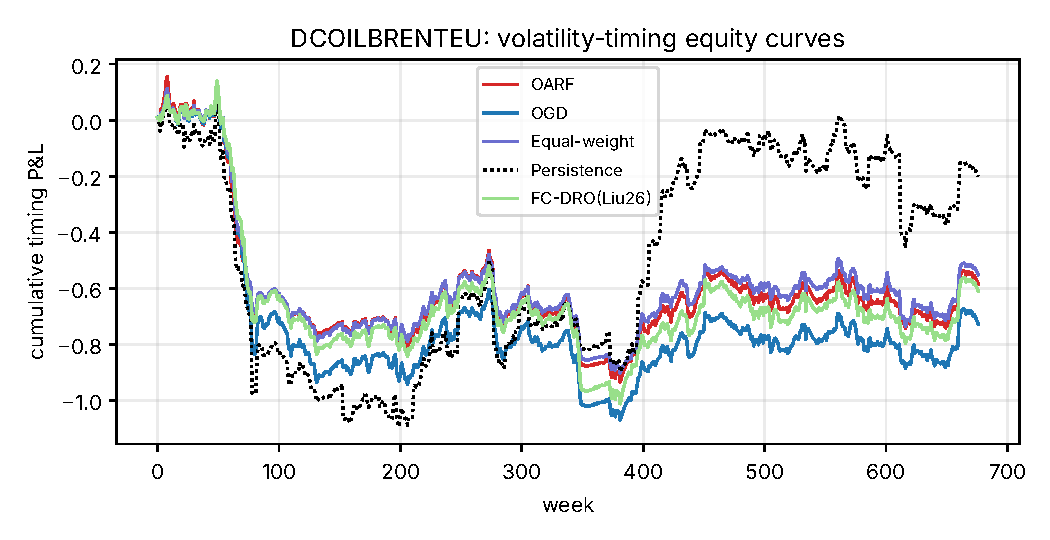
\includegraphics[width=0.66\textwidth]{fig10_equity_DCOILBRENTEU}
\caption{Brent, weekly design: cumulative volatility-timing profit and loss for
selected methods.}
\label{fig:equity}
\end{figure}

\section{Baseline implementations and notes}\label{app:baselines}
Table~\ref{tab:baseimpl} lists, for each method, the loss optimised, the update rule
and the output, whether the method runs online, rolling or in batch, and whether it uses
the anchor. All methods run under the same protocol with the hyper-parameters
of Table~\ref{tab:hyper}. Per step, the linear methods cost $O(d)$ and \OARF{} adds
$O(pq+q^3)$ for the anchor block. Rolling-OLS and the batch methods cost $O(d^3)$ at
each refit, which takes place every $5$--$10$ steps.

Some implementation details follow. The warm-up block is used only to initialise the
past-only standardiser and to select hyper-parameters once; it is never used for
separate batch pre-training. Missing FRED observations and exchange holidays are
handled by reindexing to business days with a forward-fill capped at five days, and
longer gaps are left missing and skipped. For the weekly design the daily data are
aggregated to weeks ending on Friday, and weeks with fewer than two trading days are
dropped. The GARCH$(1,1)$ expert is a
recursion with fixed coefficients ($\alpha=0.08$, $\beta=0.90$) and is never
estimated, so it uses no future data. The channel dimension is larger on the real data ($q=3$,
against $q=2$ in the synthetic experiments) because three macro-uncertainty drivers
(VIX, GPR, EPU) are chosen by hand as the anchor, while the synthetic SCM has exactly
two anchor directions by construction. We present \OARF{} for linear predictors. It
extends to nonlinear forecasters by applying the same residual--anchor penalty to a
feature map or to the top layer of a network; we leave this extension to future work.

\begin{table}[htbp]
\centering
\caption{Baseline implementations. ``Out'' = P(oint)/I(nterval); ``Mode'' =
O(nline)/R(olling)/B(atch); ``Anc'' = uses the anchor.}
\label{tab:baseimpl}
\small
\begin{tabular}{lllccc}
\toprule
Method & Loss optimised & Update rule & Out & Mode & Anc\\
\midrule
\OARF{}/\OARFCD{} & anchor-penalised sq.\ err. & AdaGrad on \eqref{eq:update} & P & O & yes\\
OGD & squared error & AdaGrad ($\xi=0$) & P & O & no\\
Rolling-OLS & windowed ridge & closed-form refit & P & R & no\\
ACI/CostACI & pinball (3 quantiles) & subgrad.\ + ACI level & P+I & O & no\\
M-FISHER & sq.\ err.\ + martingale & OGD + triggered NGD & P & O & no\\
WATCH/WCTM & sq.\ err.\ + WCTM & OGD + width adapt & P+I & O & no\\
DR-Combo & Wasserstein-DR combo & EG mirror descent & P & O & no\\
FC-DRO(-ES) & variance-/ES-scaled & exponential weights & P & O & no\\
W-DRO-OL & Wasserstein-DR sq.\ err. & primal--dual OGD & P & O & no\\
AnchorReg & anchor-penalised (batch) & windowed closed-form & P & R & yes\\
DRIG & invariant-gradient (batch) & windowed two-env.\ fit & P & R & (env)\\
\bottomrule
\end{tabular}
\end{table}

\section{Ader-wrapped versus AdaGrad OARF}\label{app:ader}
The interventional-regret theorem (Theorem~\ref{thm:main}) is stated for the
path-length-adaptive Ader step wrapper \citep{zhang2018adaptive}, whereas the deployed
model takes a single AdaGrad step. To check whether this simplification changes the
empirical behaviour, we implemented the Ader variant and compared it with the deployed
AdaGrad model on the controlled anchor-SCM (true fixed channel, $\xi=6$, $12$ seeds).
The Ader variant is a pool of five gradient-descent experts that follow the same
anchor-robust surrogate gradient with a geometric ladder of step sizes. Each expert is
projected onto the comparator ball, and a Hedge meta-learner combines them.
Table~\ref{tab:ader} reports the results. Both step rules cut the worst-case $\doop(A)$ error well below the no-anchor OGD reference, to about a third (AdaGrad) and a half (Ader) of it, and their per-seed worst-case
errors are strongly rank-correlated (Spearman $\rho=0.80$). In this experiment AdaGrad
is slightly more accurate and has lower variance. It also has fewer parameters, and for
these reasons it is the rule we deploy; the Ader wrapper is the object the theorem
analyses. Substituting one for the other leaves the qualitative ranking unchanged.

\begin{table}[htbp]
\centering
\caption{Ader-wrapped versus AdaGrad \OARF{} on the synthetic anchor-SCM ($12$ seeds,
true fixed channel, $\xi=6$; median with $[\,q_{25},q_{75}\,]$). Both reach similar
worst-case interventional error, far below the OGD reference, and their per-seed worst-case
errors are rank-correlated at Spearman $\rho=0.80$.}
\label{tab:ader}
\small
\begin{tabular}{lcc}
\toprule
Step rule & in-regime MSE & worst-$\doop(A)$ MSE\\
\midrule
AdaGrad (deployed) & $0.028$ & $0.052\,[0.030,0.114]$\\
Ader (analysed)    & $0.030$ & $0.073\,[0.026,0.142]$\\
\midrule
OGD ($\xi=0$, reference) & $0.019$ & $0.143\,[0.065,0.353]$\\
\bottomrule
\end{tabular}
\end{table}

\section{Event study: COVID-19 and the 2022 energy shock}\label{app:events}
The regime-tercile analysis of Section~\ref{sec:real} is aggregate, so here we examine
two dated episodes on the weekly design: January to September 2020 ($39$ weeks) and
calendar 2022 ($52$ weeks). We run fixed-anchor \OARF{} ($\xi=1.5$) and the no-anchor
OGD reference, and within each window we plot the cumulative squared-loss gap (\OARF{}
minus OGD, so a negative value means \OARF{} is ahead) and, for both methods, the
smoothed anchor--residual correlation $|\mathrm{corr}(a_t,r_t)|$
(Figure~\ref{fig:events}). \OARF{} is ahead in three of the four window--commodity
pairs: the COVID-19 window on Brent (cumulative gap $-0.77$) and both windows on Henry
Hub ($-1.16$ and $-2.46$). It is behind in the 2022 window on Brent ($+2.11$). In the
three windows where it leads, \OARF{} keeps the anchor--residual correlation below that
of OGD in most weeks ($67\%$, $79\%$ and $100\%$ of weeks); in the 2022 Brent window it
does so in only $4\%$ of weeks. With two episodes and no significant aggregate
difference, this is an illustration and not evidence of an advantage.

\begin{figure}[htbp]
\centering
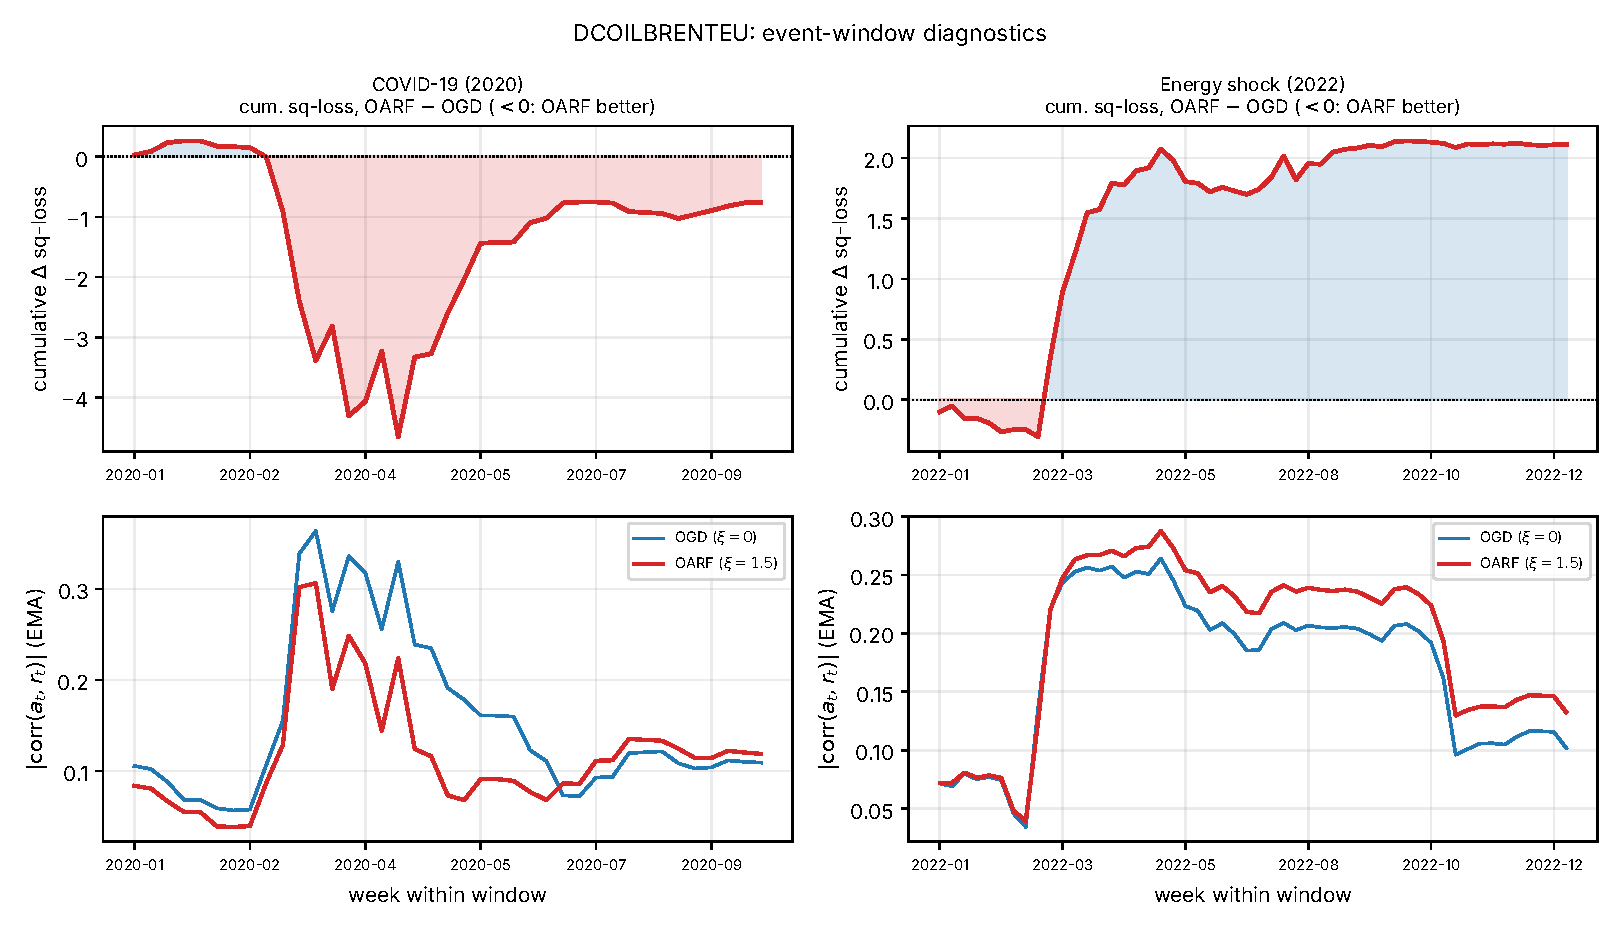
\includegraphics[width=0.96\textwidth]{fig15_events_DCOILBRENTEU}
\caption{Brent event windows, weekly design. Top: cumulative squared-loss gap,
\OARF{} minus OGD (shaded where \OARF{} leads or trails). Bottom: the smoothed
anchor--residual correlation of both methods.}
\label{fig:events}
\end{figure}

\section*{Acknowledgments}
The author used Claude (Anthropic) between June and November 2026 to help
write the analysis code and to edit the text of the manuscript. The author
reviewed and revised all code and text and takes full responsibility for the
content of this article.

\section*{Funding}
This research did not receive any specific grant from funding agencies in the
public, commercial, or not-for-profit sectors.

\section*{Conflict of interest}
The author declares no conflict of interest.

\section*{Data availability statement}
The data that support the findings of this study are openly available from the
public sources listed in Table~\ref{tab:realdata}
\citep{fred2026data,caldara2026gprdata,baker2026epudata}. The code and the scripts
that download these data and regenerate every number, table and figure are openly
available at
\url{https://github.com/vinhqdang/OARF-Online-Anchor-Robust-Forecasting-under-Economic-Regime-Shift}
\citep{dang2026oarfcode}.

\section*{Ethics approval}
Not applicable. The study uses only public, non-personal data.

\section*{Permission to reproduce material}
Not applicable. All figures and tables are original.

\small
\bibliographystyle{apalike}
\bibliography{references}

\end{document}
